\documentclass[12pt]{article}
\usepackage[utf8]{inputenc}
\usepackage[english]{babel}
\usepackage{amsmath, amsthm, amssymb, amsfonts}
\usepackage[top = 3in, left = 1in, right = 1in]{geometry}
\usepackage{hyperref}
\hypersetup{
	colorlinks=true,
	linkcolor=blue,
	filecolor=magenta,      
	urlcolor=blue,
}
\usepackage{cleveref}
\usepackage{tcolorbox}
\usepackage{bm}

% FOR TIKZ
\usepackage{tikz}
\usetikzlibrary{arrows,arrows.meta, shapes.geometric}

\usepackage{comment}


% DEFINE NEW COMMANDS AND ENVIRONMENTS
\newcommand{\R}{\mathbb{R}}
\newcommand{\C}{\mathbb{C}}
\newcommand{\N}{\mathbb{N}}
\newcommand{\Q}{\mathbb{Q}}
\newcommand{\Z}{\mathbb{Z}}
\newcommand{\transpose}{\mathsf{T}}

\newcommand{\E}{\mathbb{E}}
\newcommand{\Var}{\text{Var}}
\newcommand{\prob}{\mathbb{P}}

\newcommand{\normal}{\mathcal{N}}
\newcommand{\corr}{\mathrm{Cor}}



\newcommand{\HRule}{\rule{\linewidth}{0.5mm}} % Defines a new command for the horizontal lines, change thickness here


% DEFINE A PROBLEM Environment
\theoremstyle{definition}
\newtheorem*{prb}{Problem}
\newenvironment{problem}{\begin{tcolorbox}[colback=blue!5!white,colframe=blue!75!black, parbox = true] \begin{prb}  }{\end{prb}\end{tcolorbox} }
\newenvironment{answer}{\textit{Solution: }\quad }{ \hfill $\blacksquare$}

\numberwithin{equation}{section}


% Setting up a code writing environment
\usepackage{listings}
\usepackage{xcolor}

\definecolor{codegreen}{rgb}{0,0.6,0}
\definecolor{codegray}{rgb}{0.5,0.5,0.5}
\definecolor{codepurple}{rgb}{0.58,0,0.82}
\definecolor{backcolour}{rgb}{0.95,0.95,0.92}

\lstdefinestyle{mystyle}{
    backgroundcolor=\color{backcolour},   
    commentstyle=\color{codegreen},
    keywordstyle=\color{magenta},
    numberstyle=\tiny\color{codegray},
    stringstyle=\color{codepurple},
    basicstyle=\ttfamily\footnotesize,
    breakatwhitespace=false,         
    breaklines=true,                 
    captionpos=b,                    
    keepspaces=true,                 
    numbers=left,                    
    numbersep=5pt,                  
    showspaces=false,                
    showstringspaces=false,
    showtabs=false,                  
    tabsize=2
}

\lstset{style=mystyle}



\begin{document}


% TITLE PAGE
%%%%%%%%%%%%%%%%%%%%%%%%%%%%%%%%%%%%%%%%%%%%%%%%%%%%%%
\begin{titlepage}
    
\centering
\textsc{\LARGE Indian Statistical Institute, Kolkata}\\[1.5cm] % Name of your university/college
\textsc{\Large Large Sample Statistical Methods}\\[0.5cm] % Major heading such as course name
\textsc{\large End Semestral Examinations 2019-2020}\\[0.5cm] % Minor heading such as course title

\HRule \\[0.4cm]
\large \textbf{Subhrajyoty Roy}\\
\large \textbf{Roll:  MB1911}\\
\HRule \\[1.5cm]
\normalsize \today

\end{titlepage}


\tableofcontents
\clearpage


% CONTENT FROM HERE
%%%%%%%%%%%%%%%%%%%%%%%%%%%%%%%%%%%%%%%%%%%%%%%%%%
\newgeometry{margin = 1in}


\textbf{Note}: \textit{$X,X_n,Y_n (n\geq 1)$ denote random variables. For any limiting distribution we assume $n\rightarrow \infty$.}

\section{Problem 1}
\begin{problem}
Let $X,X_n,n\geq 1$, be random variables such that
$$\lim\inf_{n\rightarrow\infty}\E\left[g(X_n)\right] \geq \E\left[g(X)\right]$$
for every bounded continuous function $g:(-\infty,\infty)\rightarrow[0,\infty)$. Show that, $X_n\xrightarrow{d}X$. [It is known that $X_n\xrightarrow{d}X$ if and only if $\displaystyle\lim_{n\rightarrow\infty}\E\left[g(X_n)\right]=\E\left[g(X)\right]$ for every bounded continuous function $g:\R\rightarrow\R$.\big] 
\end{problem}

\begin{answer}
    
    We are given $X,X_n,n\geq 1$, be random variables such that 

    \begin{equation}
        \lim\inf_{n\rightarrow\infty}\E\left[g(X_n)\right] \geq \E\left[g(X)\right]
        \label{eqn:1-1}
    \end{equation}
    
    for every bounded continuous function $g:(-\infty,\infty)\rightarrow[0,\infty)$. 
    
    Let, $g : \R \rightarrow [0, \infty)$ be any bounded and continuous function. Since $g$ is bounded, there must exist $M > 0$ such that, $g(x) \leq M \quad \forall x \in \R$. Consider the function $g'(x) = M - g(x)$, clearly, $g': \R \rightarrow [0, \infty)$, and is continuous and is also bounded, (as $g'(x) \leq M$ since $g(x) \geq 0$). Therefore, by applying \cref{eqn:1-1} on $g'$ instead of $g$ it follows that:

    \begin{align*}
        & \lim \inf_{n \rightarrow \infty} \E\left[ g'(X_n) \right] \geq \E\left[ g'(X) \right]\\
        \implies \quad & \lim\inf_{n \rightarrow \infty} \E\left[ M - g(X_n) \right] \geq \E\left[ M - g(X) \right]\\
        \implies \quad & M - \lim\sup_{n \rightarrow \infty} \E\left[ g(X_n)\right] \geq M - \E\left[ g(X) \right] \\
        \implies \quad & \E\left[ g(X) \right] \geq \lim\sup_{n \rightarrow \infty} \E\left[ g(X_n)\right]
    \end{align*}

    Thus, combining this and \cref{eqn:1-1} yields,

    $$
    \lim\inf_{n \rightarrow \infty}\E\left[g(X_n) \right] \geq \E\left[g(X)\right] \geq \lim\sup_{n \rightarrow \infty} \E\left[ g(X_n) \right]
    $$

    but as limit superior of a sequence must be atleast as large as the limit inferior, equality must hold throughout and the limit of the sequence $\E\left[g(X_n)\right]$ must exists.


    Thus we obtain that for any such bounded and continuous function $g : \R \rightarrow [0, \infty)$, the limit infimum in \cref{eqn:1-1} can actually be replaced by limit while the inequality can be replaced by an equality, i.e.

    \begin{equation}
        \lim_{n \rightarrow \infty} \E\left[ g(X_n) \right] = \E\left[g(X)\right]
        \label{eqn:1-2}
    \end{equation}

    holds for any bounded and continuous positive valued function $g$.
    

    We know that, $X_n \xrightarrow{d} X$ if and only if \cref{eqn:1-2} holds for every bound and continuous function $g : \R \rightarrow \R$, hence it is enough to show that \cref{eqn:1-2} holds for all such functions.


    Consider such a function $h : \R \rightarrow \R$ such that $\lim_{n\rightarrow\infty}\E\left[h(X_n)\right]=\E\left[h(X)\right]$. Define the positive and negative part of the function as follows:

    $$
    h_{+}(x) = \begin{cases}
        h(x) & \text{ if } h(x) \geq 0\\
        0 & \text{ if } h(x) < 0
    \end{cases}
    $$

    and 

    $$h_{-}(x)=\begin{cases}
        -h(x) & \text{ if } h(x)\leq 0\\
        0 & \text{ otherwise}
    \end{cases}
    $$
    
Now observe that, $h_{+} : \R \rightarrow [0, \infty)$, $h_{-} : \R \rightarrow [0, \infty)$ and $h(x)=h^+(x)-h^-(x)\quad \forall x\in\R$. Also note that, $h_{+}(x) = \max\{ h(x), 0 \}$ and $h_{-}(x) = -\min\{ h(x), 0 \}$ for any $x \in \R$. Since, $h$ is chosen to be bounded and continuous, so is $h_{+}$ and $h_{-}$.

Hence, as $h_{+}$ and $h_{-}$ are positive valued function, by the limit in \cref{eqn:1-2} we get that,

$$ 
\lim_{n\rightarrow\infty}\E\left[h_{+}(X_n)\right] = \E\left[h_{+}(X)\right]\quad \text{and} \quad \lim_{n\rightarrow\infty}\E\left[h_{-}(X_n)\right] = \E\left[h_{-}(X)\right]
$$

Note that, the above expectations exist because it is assumed that $\E(h(X))$ and $\E(h(X_n))$ exist and thus $\E[\vert h(X) \vert]$ and $\E[\vert h(X_n)\vert]$ exist.


Finally we have,

\begin{align*}
    \lim_{n\rightarrow\infty}\E\left[h(X_n)\right] 
    & = \lim_{n\rightarrow\infty}\E\left[h_{+}(X_n)+h_{-}(X_n)\right]\\
    & = \lim_{n\rightarrow\infty}\left[\E\left[h_{+}(X_n)\right]+ \E\left[h_{-}(X_n)\right] \right] \quad \text{by linearity of expectation}\\
    & = \lim_{n\rightarrow\infty}\E\left[h_{+}(X_n)\right]+\lim_{n\rightarrow\infty} \E\left[h_{-}(X_n)\right] \\
    & = \E\left[h_{+}(X)\right] + \E\left[h_{-}(X)\right] \quad \text{by } \cref{eqn:1-1}\\
    & = \E\left[h_{+}(X)+h_{-}(X)\right]\\
    & = \E\left[ h(X) \right]
\end{align*}

\begin{equation}
    \therefore \lim_{n\rightarrow\infty}\E\left[h(X_n)\right] = \E\left[h(X)\right] 
    \label{eqn:1-3}
\end{equation}

Since, \cref{eqn:1-3} holds for any $h : \R \rightarrow \R$ being bounded and continuous function, by Portmanteau's theorem, it follows that $X_n \xrightarrow{d} X$.

This completes the proof.


\end{answer}

\pagebreak
\section{Problem 2}
\begin{problem}
If $X_n \xrightarrow{p} 0$, show that for any median $M_n$ of $X_n$, $M_n\rightarrow 0$.
\end{problem}

\begin{answer}


We are given that, $X_n \xrightarrow{P} 0$. We consider any median $M_n$ of $X_n$. We shall prove that $M_n \rightarrow 0$ as $n \rightarrow \infty$, by method of contradiction.

For the sake of contradiction, we start by assuming that $M_n \not\rightarrow 0$. This means, there exists $\epsilon > 0$ such that, for any $n \in \N$, there is an even bigger integer $a_n > n$ such that $\vert M_{a_n} \vert > \epsilon$.

Now consider the sequence $\{a_n\}_{n = 1}^{\infty}$. As $M_{a_n}$'s are medians of respective $X_{a_n}$'s, we have;

\begin{equation}
    \prob\left( X_{a_n} \geq M_{a_n} \right)\geq \dfrac{1}{2}\quad \text{and}\quad \prob\left( X_{a_n} \leq M_{a_n} \right)\geq \dfrac{1}{2}
    \label{eqn:2-1}
\end{equation}

Now we consider two cases separately.

\begin{enumerate}
    \item \textbf{Case 1:} $M_{a_n} > 0$. Since, $a_n$'s are such that $\vert M_{a_n} \vert > \epsilon$, we must have $M_{a_n} > \epsilon$. Now, 
    
    $$\left\{ w: X_{a_n}(w) \geq M_{a_n} \right\} \subseteq \left\{ w: X_{a_n}(w) \geq \epsilon \right\} \subseteq \left\{ w: \vert X_{a_n}(w)\vert \geq \epsilon \right\}$$

    Therefore using \cref{eqn:2-1},

    \begin{equation}
        \dfrac{1}{2}\leq \prob\left( X_{n_N} \geq M_{n_N} \right) \leq \prob\left( |X_{n_N}|>\epsilon\right)
        \label{eqn:2-2}
    \end{equation}

    \item \textbf{Case 2:} $M_{a_n} < 0$. Similar to the previous case, $M_{a_n} < 0 \implies M_{a_n} < -\epsilon$. Hence,
    
    $$\left\{ w: X_{a_n}(w) \leq M_{a_n} \right\} \subseteq \left\{ w: X_{a_n}(w) \leq -\epsilon \right\} \subseteq \left\{ w: \vert X_{a_n}(w)\vert \geq \epsilon \right\}$$

    Therefore using \cref{eqn:2-1},

    \begin{equation}
        \dfrac{1}{2}\leq \prob\left( X_{n_N} \leq M_{n_N} \right) \leq \prob\left( |X_{n_N}|>\epsilon\right)
        \label{eqn:2-3}
    \end{equation}

\end{enumerate}

So, now by combining \cref{eqn:2-2} and \cref{eqn:2-3}, we get,

$$\prob\left( |X_{n_N}|>\epsilon\right)\geq \dfrac{1}{2} \quad \forall a_n, n \in \N$$

i.e. 

$$\prob\left( |X_{n_N}|>\epsilon\right) \not\rightarrow 0$$

which contradicts the fact that $X_n \xrightarrow{P} 0$.
\end{answer}

\pagebreak
\section{Problem 3}

\begin{problem}
 Let $X_1,X_2,\cdots,X_n$ be a random sample from a distribution with a density $f(x, \theta)$ where $\theta$ is an unknown real parameter. Give an example to show that there may exist a consistent estimator $T_n$ of $\theta$ for which $\E(T_n) \rightarrow\theta + 1$ as $n\rightarrow\infty$. [\textbf{Hint}: Consider an example where there is an unbiased consistent estimator $\hat{\theta}_n$ and a set $A_n$, independent of $\hat{\theta}_n$, with probability tending to one and with some other property so that $\hat{\theta}_n$ can be modified with the help of $A_n$ to construct $T_n$.]
\end{problem}

\begin{answer}

Let us consider a specific density, namely the density of the normal distribution. Let $X_1,X_2,\cdots,X_n$ be independent and identically distributed random sample from a normal distribution $\normal(\theta, 1)$, where $\theta$ is an unknown and $\theta \in \R$. 

Now, denoting $\bar{X}_n$ as the sample mean, i.e. $\overline{X_n} = \dfrac{1}{n} \sum_{i=1}^{n} X_i$, consider the set $A_n = \left\{ w : \vert X_{1} - \bar{X}_n \vert \leq \sqrt{n} \right\}$. Clearly, $\bar{X}_n$ is independent of the statistic $\vert X_{1} - \bar{X}_n \vert$, hence in effect, the set $A_n$ becomes independent of the estimator $\bar{X}_n$, as suggested by the hint given in the question.

Consider the estimator which modifies the estimator $\bar{X}_n$ with the help of the set $A_n$ appropriately,

$$T_n = \bar{X}_n \bm{1}_{A_n} + (\bar{X}_n + \delta_n) \bm{1}_{A_n^c}$$

where $\bm{1}_A$ is the indicator function of $A$ and 

$$
\delta_n = \dfrac{1}{2}\left[ 1 - \Phi\left( \dfrac{n}{\sqrt{(n-1)}}\right) \right]^{-1} \forall n \geq 2 \qquad \text{ and } \qquad \delta_1 = 1
$$

As the set $A_n$ depends on the sample $X_1, \dots X_n$ rather than some randomization device, it belongs to the same measure space as the space of functions of the samples. Thus, the given probability measure can be used to calculate appropriate probabilities and expectations regarding $T_n$ without any problem. 

First, note that, $\bar{X}_n \xrightarrow{P} \theta$, by Weak Law of Large Numbers, hence is consistent for $\theta$. 


Now, we shall show that $(T_n - \bar{X}_n) \xrightarrow{P} 0$. To show this, choose any sufficiently small $\epsilon > 0$, and consider the following probability;

\begingroup
\allowdisplaybreaks
\begin{align*}
    \prob_\theta(\vert T_n - \bar{X}_n \vert > \epsilon)
    & \leq \prob_\theta( T_n \neq \bar{X}_n ) \\
    & = \prob_\theta(A_n^c) \qquad \text{, since } \delta_n > 0 \quad\forall n \geq 1 \text{ and } \lim_{n \rightarrow \infty} \delta_n > 0\\
    & = \prob_\theta\left( \vert X_1 - \bar{X}_n \vert > \sqrt{n} \right)\\
    & = 2 \prob_\theta\left( (X_1 - \bar{X}_n) > \sqrt{n} \right) \qquad \text{, since } X_1 - \bar{X}_n \text{ has a symmetric distribution about 0}\\
    & = 2 \prob_\theta\left( \dfrac{\sqrt{n}}{\sqrt{(n-1)}} (X_1 - \bar{X}_n) > \dfrac{n}{\sqrt{(n-1)}} \right)\\
    & = 2 \left(1 - \Phi\left( \dfrac{n}{\sqrt{(n-1)}} \right)\right) \qquad \text{, since } (X_1 - \bar{X}_n) \sim \normal(0, 1-1/n)\\
    & \qquad \qquad \qquad \text{, where } \Phi(\cdot) \text{ is the cdf of standard normal distribution}\\  
    & \rightarrow 0, \quad \text{as } n \rightarrow \infty
\end{align*}
\endgroup

where the limit in the last line follows from the fact that $\Phi(\cdot)$ is a continuous function and $\Phi(x) \rightarrow 1$ as $x \rightarrow \infty$. Therefore, we have $(T_n - \bar{X}_n) \xrightarrow{P} 0$, and hence, 

$$T_n = (T_n - \bar{X}_n) + \bar{X}_n \xrightarrow{P} \theta$$

Thus, $T_n$ is a consistent estimator for $\theta$.

On the other hand,
 
\begin{align*}
    \E_\theta(T_n) 
    & = \E_\theta\left( \bar{X}_n \bm{1}_{A_n} + (\bar{X}_n + \delta_n)\bm{1}_{A_n^c} \right)\\
    & = \E_\theta\left( \bar{X}_n (\bm{1}_{A_n} + \bm{1}_{A_n^c}) + \delta_n \bm{1}_{A_n^c} \right)\\
    & = \E_\theta\left( \bar{X}_n + \delta_n \bm{1}_{A_n^c} \right) \qquad \text{, since } \bm{1}_{A_n} + \bm{1}_{A_n^c} = 1\\
    & = \E_\theta\left( \bar{X}_n \right) + \delta_n \E_\theta\left( \bm{1}_{A_n^c} \right) \quad \text{, by linearity of expectation}\\
    & = \theta + \delta_n \prob_\theta(A_n^c) \quad \text{, since } \E(\bm{1}_A) = \prob(A)\\
    & = \theta + 2\delta_n \left( 1 - \Phi\left( \dfrac{n}{\sqrt{(n-1)}}\right) \right) \qquad \text{, by the previously shown derivations}\\
    & = \theta + 1 \quad \forall n \geq 2 
\end{align*}

where the last equality follows from the definition of $\delta_n$, which was chosen in a particular way to ensure this multiplication becomes 1. Thus, $\E_{\theta}(T_n) \rightarrow \theta+1$ as $n \rightarrow \infty$. 


Thus we have obtained a consistent estimator $T_n$ of $\theta$ for which $\E(T_n) \rightarrow\theta + 1$.
\end{answer}

\pagebreak
\section{Problem 4}

\begin{problem}
Suppose that $(X_i,Y_i),i\geq 1$ are i.i.d. bivariate random vectors with $\E(X_1)=\mu_x,\E(Y_1)=\mu_y,\Var(X_1)=\sigma_x^2,\Var(Y_1)=\sigma_y^2$ and $\corr(X_1,Y_1)=\rho$. If $X_i$ and $Y_i$ are positive random variables, using univariate Central Limit Theorem (CLT) show that

$$\sqrt{n}\left( \dfrac{\sum_{i=1}^n X_i}{\sum_{i=1}^n Y_i} - \dfrac{\mu_x}{\mu_y} \right)$$

converges in distribution to a normal random variable with mean $0$ and variance 
$\left( \mu_y^2\sigma_x^2 + \mu_x^2\sigma_y^2 - 2\rho\mu_x\mu_y\sigma_x\sigma_y \right)/\mu_y^4$. 
(Note that one can use multivariate CLT and delta method to find the asymptotic distribution. You have been asked to use univariate CLT).
\end{problem}

\begin{answer}

We are given $(X_i,Y_i),i\geq 1$ are i.i.d. bivariate random vectors with $\E(X_1)=\mu_x,\E(Y_1)=\mu_y,\Var(X_1)=\sigma_x^2,\Var(Y_1)=\sigma_y^2$ and $\corr(X_1,Y_1)=\rho$. 

We start by simplying the given quantity;

\begin{align*}
    \dfrac{\sum_{i=1}^n X_i}{\sum_{i=1}^n Y_i} - \dfrac{\mu_x}{\mu_y} 
    & =\dfrac{1}{\sum_{i=1}^n Y_i}\left( \sum_{i=1}^n X_i- \dfrac{\mu_x}{\mu_y} \sum_{i=1}^n Y_i \right)\\
    & =\dfrac{\sum_{i=1}^n\left(  X_i- \dfrac{\mu_x}{\mu_y} Y_i \right)}{\sum_{i=1}^n Y_i}\\
    & = \dfrac{\sum_{i=1}^{n} Z_i}{\sum_{i = 1}^{n} Y_i} \qquad \text{, where } Z_i =X_i- \dfrac{\mu_x}{\mu_y} Y_i, \quad \forall i = 1, 2, \dots n\\
    & = \dfrac{\sum_{i=1}^{n} Z_i / n}{\sum_{i=1}^{n} Y_i / n}\\
    & = \dfrac{\overline{Z_n}}{\overline{Y_n}} \qquad \text{, where } \overline{Z_n} = \dfrac{1}{n} \sum_{i=1}^n Z_i \text{ and similarly } \overline{Y_n} = \dfrac{1}{n} \sum_{i=1}^n Y_i
\end{align*}

Now since $X_i, Y_i$'s are i.i.d. bivariate normal random variables, being a linear combination of them, $Z_i$'s are also i.i.d. normal random variables. Note that,

\begin{align*}
    \E(Z_i) & = \E(X_i)- \dfrac{\mu_x}{\mu_y} \E(Y_i)\\
    & = \mu_x- \dfrac{\mu_x}{\mu_y} \mu_y\\
    & = 0
\end{align*}

and,

\begin{align*}
    \Var(Z_i)& =\Var(X_i)- \dfrac{\mu_x^2}{\mu_y^2} \Var(Y_i) - 2\dfrac{\mu_x}{\mu_y} \text{Cov}(X_i,Y_i)\\
    & = \sigma_x^2- \dfrac{\mu_x^2}{\mu_y^2} \sigma_y^2 - 2\dfrac{\mu_x}{\mu_y}\rho \sigma_x\sigma_y\\
    & = \dfrac{1}{\mu_y^2}\left[ \mu_y^2\sigma_x^2 + \mu_x^2\sigma_y^2 - 2\rho\mu_x\mu_y\sigma_x\sigma_y \right]\\
    & = \dfrac{S}{\mu_y^2}\quad \left[\text{Let, } S = \mu_y^2\sigma_x^2 + \mu_x^2\sigma_y^2 - 2\rho\mu_x\mu_y\sigma_x\sigma_y\right]
\end{align*}

Now, using Univariate Central Limit Theorem (CLT) on these $Z_i$'s, we obtain,

\begin{align*}
    \sqrt{n}(\overline{Z_n}-0)\xrightarrow{d}\normal\left(0,\dfrac{S}{\mu_y^2}\right)\\
    \text{i.e.,}\quad \sqrt{n}\bar{Z_n}\xrightarrow{d}\normal\left(0,\dfrac{S}{\mu_y^2}\right)
\end{align*}

Again, by using Weak Law of Large Numbers, it follows that,

\begin{align*}
    \dfrac{1}{n}\sum_{i=1}^n Y_i & \xrightarrow{P} \mu_y\\
    \text{i.e.,}\quad \overline{Y_n} & \xrightarrow{P} \mu_y,\text{ which is a constant.} 
\end{align*}

So, by Slutsky's Theorem, we have, 

\begin{align*}
    \sqrt{n}\left(\dfrac{\overline{Z_n}}{\overline{Y_n}}\right) 
    & \xrightarrow{d} \dfrac{W}{\mu_y} \qquad \text{, where } W \sim \normal\left(0,\dfrac{S}{\mu_y^2}\right)\\
    \text{i.e.,}\quad  \sqrt{n}\left( \dfrac{\sum_{i=1}^n X_i}{\sum_{i=1}^n Y_i} - \dfrac{\mu_x}{\mu_y} \right) 
    & \xrightarrow{d}\normal\left(0,\dfrac{\mu_y^2\sigma_x^2 + \mu_x^2\sigma_y^2 - 2\rho\mu_x\mu_y\sigma_x\sigma_y}{\mu_y^4}\right) 
\end{align*}

This is what we intended to show.

\end{answer}

\pagebreak
\section{Problem 5}


\begin{problem}
Let $X_1,X_2,\cdots,X_n$ be a random sample from a distribution with mean $\mu$, variance $\sigma^2$ and finite $4^{th}$ moment $\mu_4$. A common test for $H_0 :\sigma^2= 1$ versus $H_1 :\sigma^2> 1$ rejects $H_0$ when 
$$nS_n^2 = \displaystyle\sum_{i=1}^n \left(X_i-\bar{X}_n\right)^2 > \chi_{\alpha,n-1}^2$$
where $\chi_{\alpha,n-1}^2$ is the upper $\alpha$ point of a central chi-square distribution with $(n-1)$ degrees of freedom. Show that $\prob_{H_0}\left( nS_n^2 > \chi_{\alpha,n-1}^2 \right)$ converges to $\alpha$ as $n \rightarrow\infty$ only if the value of the kurtosis $\kappa = \dfrac{\mu_4}{\sigma^4}-3$ is equal to zero. [\textbf{Hint}: First show (using the CLT and Polya’s Theorem) that $ \dfrac{\chi_{\alpha,n-1}^2-(n-1)}{\sqrt{2n-2}}$ converges to the upper $\alpha$ point $z_\alpha$ of the standard normal distribution.]
\end{problem}

\begin{answer}
    Let, $Y_1, Y_2, \dots Y_{(n-1)}$ be i.i.d. random sample from a standard normal distribution. Then, $T_n = \sum_{i=1}^{(n-1)}Y_i^2$ has a chi-squared distribution with $(n-1)$ degrees of freedom.

    Note that, $\E(T_n) = \sum_{i=1}^{(n-1)} \E(Y_i^2) = \sum_{i=1}^{(n-1)} (\Var(Y_i^2) + \E(Y_i)^2) = (n-1)$. Also, 

    $$
    \Var(T_n) = \sum_{i=1}^{(n-1)} \Var(Y_i^2) = \sum_{i=1}^{(n-1)} (\E(Y_i^4) - \E(Y_i^2)^2) = (n-1)(3-1) = (2n-2)
    $$

    Therefore, an application of Central Limit Theorem yields,

    $$\dfrac{T_n - (n-1)}{\sqrt{2n - 2}} \xrightarrow{d} Z \sim N(0, 1)$$

    Now, choose any $\epsilon > 0$. Then by using Polya’s theorem, it follows that for large $n$, say $\forall n \geq N_1$, 

    \begin{equation}
        \left\vert \prob\left( \dfrac{T_n - (n-1)}{\sqrt{2n - 2}} \leq \dfrac{\chi^2_{\alpha, (n-1)} - (n-1)}{\sqrt{2n - 2}} \right) - \prob\left( Z \leq \dfrac{\chi^2_{\alpha, (n-1)} - (n-1)}{\sqrt{2n - 2}} \right) \right\vert < \epsilon
        \label{eqn:5-1}        
    \end{equation}

    However, since $\chi^2_{\alpha, (n-1)}$ is the upper $\alpha$-quantile of chi-squared distribution with $(n-1)$ degrees of freedom and $T_n$ is a random variable following chi-squared distribution with $(n-1)$ degrees of freedom, we have;

    \begin{equation}
        \prob\left( \dfrac{T_n - (n-1)}{\sqrt{2n - 2}} \leq \dfrac{\chi^2_{\alpha, (n-1)} - (n-1)}{\sqrt{2n - 2}} \right) = \prob(T_n \leq \chi^2_{\alpha, (n-1)}) = (1-\alpha)
        \label{eqn:5-2}
    \end{equation}

    Since $(1 - \alpha) = \prob(Z \leq z_\alpha)$, combining \cref{eqn:5-1} and \cref{eqn:5-2}, we obtain;

    \begin{equation}
        \left\vert \prob\left( Z \leq \dfrac{\chi^2_{\alpha, (n-1)} - (n-1)}{\sqrt{2n - 2}} \right) -\prob(Z \leq z_\alpha) \right\vert < \epsilon \qquad \forall n \geq N_1
        \label{eqn:5-3}
    \end{equation}

    Letting $\Phi(\cdot)$ denote the cumulative distribution function of a standard normal distribution, \cref{eqn:5-3} means that,

    $$
    \Phi\left( \dfrac{\chi^2_{\alpha, (n-1)} - (n-1)}{\sqrt{2n - 2}} \right) \xrightarrow{n \rightarrow \infty} \Phi(z_\alpha)
    $$

    Now, since $\Phi(\cdot)$ is strictly increasing and continuous, thus $\Phi^{-1}(\cdot)$ exists and is continuous. Applying $\Phi^{-1}(\cdot)$ to both sides of the above limit thus yields,

    \begin{equation}
        \dfrac{\chi^2_{\alpha, (n-1)} - (n-1)}{\sqrt{2n - 2}} \xrightarrow{n\rightarrow \infty} z_\alpha
        \label{eqn:5-4}
    \end{equation}

    Let us now consider the centered samples, $Z_i = (X_i - \mu)$. Then, 
    
    \begin{align*}
        \E(Z_i) & = \E(X_i) - \mu = 0\\
        \E(Z_i^2) & = \Var(Z_i) + \E^2(Z_i) = \Var(X_i) + 0 = \sigma^2\\
        \Var(Z_i^2) & = \E(Z_i^4) - \E^2(Z_i^2) = \mu_4 - \sigma^4\\       
    \end{align*}

    Therefore, by using Central Limit Theorem (CLT) it follows that;

    \begin{equation*}
        \sqrt{n} \dfrac{n^{-1}\sum_{i=1}^{n} Z_i^2 - \sigma^2}{\sqrt{\mu_4 - \sigma^4}} \xrightarrow{d} \normal(0, 1)
    \end{equation*}

    However, note that, $\sum_{i=1}^{n} Z_i^2 = nS_n^2 + n(\bar{X}_n - \mu)^2$. Hence, the above can be rewritten as;

    \begin{equation}
        \sqrt{n}  \left[\dfrac{S_n^2 + (\bar{X}_n - \mu)^2 - \sigma^2}{\mu_4 - \sigma^4}\right] \xrightarrow{d} \normal(0, 1)
        \label{eqn:5-5}
    \end{equation}
    
    Also, by Chebyshev's inequality,

    \begin{align*}
        \prob_{H_0}(\sqrt{n} (\bar{X}_n - \mu)^2 > \epsilon)
        & = \prob_{H_0}\left( \vert \bar{X}_n - \mu \vert > \dfrac{\epsilon^{1/2}}{n^{1/4}} \right)\\
        & \leq \dfrac{\Var_{H_0}(\bar{X}_n - \mu)}{\left(\epsilon^{1/2} / n^{1/4} \right)^2}\\
        & = \dfrac{\sigma^2}{n} \times \dfrac{\sqrt{n}}{\epsilon}\\
        & = \dfrac{\sigma^2}{\epsilon\sqrt{n}}\\
        & \rightarrow 0  \qquad \text{as, } n \rightarrow \infty
    \end{align*}

    Thus, $\sqrt{n}(\bar{X}_n - \mu)^2 \xrightarrow{P} 0$ under $H_0$. From \cref{eqn:5-5}, by an application of Slutsky's theorem, we obtain;

    \begin{equation*}
         \sqrt{n}  \left[\dfrac{S_n^2 + (\bar{X}_n - \mu)^2 - \sigma^2}{\sqrt{\mu_4 - \sigma^4}}\right] - \left[\dfrac{\sqrt{n}(\bar{X}_n - \mu)^2}{\sqrt{\mu_4 - \sigma^4}}\right]
         = \sqrt{n}  \left[\dfrac{S_n^2 - \sigma^2}{\sqrt{\mu_4 - \sigma^4}}\right] \xrightarrow{d} \normal(0, 1)
    \end{equation*}

    i.e.

    \begin{equation}
        \sqrt{n} \dfrac{\left((S_n^2/\sigma^2) - 1\right)}{\sqrt{\kappa + 2}} \xrightarrow{d} \normal(0, 1)
        \label{eqn:5-6}
    \end{equation}

    where $\kappa = \left(\dfrac{\mu_4}{\sigma^4} - 3\right)$ is the population kurtosis.

    Now, under $H_0: \sigma^2 = 1$, 

    \begin{equation}
        \dfrac{(nS_n^2 - (n-1))}{\sqrt{2(n-1)}}
        = \sqrt{n} \dfrac{\left( (S_n^2/\sigma^2)  - 1\right)}{\sqrt{\kappa + 2}} \times \dfrac{\sqrt{n}\sqrt{\kappa + 2}}{\sqrt{2(n-1)}} + \dfrac{1}{\sqrt{2(n-1)}}
        \label{eqn:5-7}
    \end{equation}

    As, $\dfrac{\sqrt{n}\sqrt{\kappa + 2}}{\sqrt{2(n-1)}} \rightarrow \sqrt{\dfrac{\kappa + 2}{2}}$ and $\dfrac{1}{\sqrt{2(n-1)}} \rightarrow 0$, combining \cref{eqn:5-6} and \cref{eqn:5-7}, it follows that 

    \begin{equation}
        \dfrac{(nS_n^2 - (n-1))}{\sqrt{2(n-1)}} \xrightarrow{d} \normal\left( 0, \dfrac{\kappa + 2}{2} \right)
        \qquad \text{ under } H_0
        \label{eqn:5-8}
    \end{equation}

    Hence,

    \begin{align*}
        \prob_{H_0}\left( nS_n^2 > \chi^2_{\alpha, (n-1)} \right)
        & = \prob_{H_0} \left( \dfrac{(nS_n^2 - (n-1))}{\sqrt{2(n-1)}} > \dfrac{(\chi^2_{\alpha, (n-1)} - (n-1))}{\sqrt{2(n-1)}} \right)\\
        & \rightarrow \prob_{H_0}\left( Z > z_\alpha \right)
        \qquad \text{where } Z \sim \normal\left( 0, \dfrac{\kappa + 2}{2} \right)\\
        & \qquad \text{ the limit follows from Polya’s theorem and \cref{eqn:5-4}}\\
        & = \prob_{H_0} \left( \sqrt{\dfrac{2}{\kappa + 2}}Z > \sqrt{\dfrac{2}{\kappa + 2}} z_\alpha \right), \quad \text{ where } \sqrt{\dfrac{2}{\kappa + 2}}Z \sim \normal(0, 1)
    \end{align*}

    Since the limit of a sequence of real numbers is unique, thus $P_{H_0}(nS_n^2 > \chi^2_{\alpha, (n-1)})$ converges to $\alpha$ as $n \rightarrow \infty$ only if $\sqrt{\dfrac{2}{\kappa + 2}} z_\alpha$ is the upper $\alpha$ quantile of standard normal distribution. However, definition $z_\alpha$ is the upper $\alpha$ quantile and as standard normal distribution function is strictly increasing, each quantile is unique. Thus, the limit holds only if $\sqrt{\dfrac{2}{\kappa + 2}} = 1$, i.e. $\kappa = 0$, i.e the kurtosis is equal to 0.

    Therefore, it follows that $\prob_{H_0}\left( nS_n^2 > \chi^2_{\alpha, (n-1)} \right) \rightarrow \alpha$ only if the kurtosis is equal to 0.
\end{answer}


\pagebreak
\section{Problem 6}

\begin{problem}
\textit{Simulation experiment.} 
\begin{itemize}
    \item[(a)] For $n = 20$ and $30$, draw $1000$ random samples of size $n$ from a bivariate normal distribution $\normal_2(0, 0, 1, 1, \rho)$ for $\rho = 0.2, 0.4, 0.6, 0.8$. Tabulate the estimated coverage probabilities of the (approximate) confidence intervals for $\rho$ formed using the $\tanh^{-1}$ transformation of the correlation coefficient.
    
    \item[(b)] Plot the histogram of the $1000$ sample correlation coefficents $r_n$’s for $n = 30$ and $\rho = 0.4$ and also the histogram of the corresponding $\tanh^{-1}r_n$’s.
\end{itemize}
\end{problem}

\begin{answer}

    \begin{enumerate}
        \item[(a)] We know that based on Fisher's $\tanh^{-1}$ transformation, an asymptotic distribution of the transformed sample correlation coefficient can be obtained as;
    
        $$\sqrt{n}( \tanh^{-1}(r_n) - \tanh^{-1}(\rho) ) \xrightarrow{d} \normal(0, 1)$$
    
        where $r_n$ is the sample correlation coefficent based on a sample of size $n$. Thus, an approximate asymptotic $95\%$ confidence interval is;
        
        $$\left( \tanh\left( \tanh^{-1}(r_n) - \dfrac{z_{0.975}}{\sqrt{n}} \right), \tanh\left( \tanh^{-1}(r_n) + \dfrac{z_{0.975}}{\sqrt{n}} \right) \right)$$
    
        To obtain the coverage probabilities, we consider $B$ monte carlo simulations, and for each simulation, we generate random samples from bivariate random sample and check whether the above confidence interval contains the population correlation coefficent $\rho$.

        First, we shall create a function for computing $\tanh^{-1}(\cdot)$.

        \begin{lstlisting}[language = R]
tanhinv <- function(r) {
    return(1/2 * log((1+r)/(1-r)))
}\end{lstlisting}

        Next, we create a function that performs $B = 1000$ monte carlo simulations to estimate the coverage probabilities. For reproducibility, I have set a seed \texttt{1911} with \texttt{R version 3.6.3} and OS platform \texttt{x86\_64-w64-mingw32} in Windows 10.

\begin{lstlisting}[language = R]
    estimate.coverage <- function(n, rho) {
    # set a seed for reproducibility
    set.seed(1911)
    
    # create the parameters
    mu_vec <- c(0, 0)
    sigma_mat <- matrix(c(1, rho, rho, 1), nrow = 2, byrow = TRUE)
    coverage <- logical(1000)  # a logical array to see if the coverage happens
    
    # loop through each simulation
    for (i in 1:1000) {
        data <- MASS::mvrnorm(n = n, mu = mu_vec, Sigma = sigma_mat)
        r <- cor(data[, 1], data[, 2])   # sample correlation coefficient
        z <- tanhinv(r)  # obtain tanh inverse transformation of sample correlation
        z.upper <- tanh(z + qnorm(0.975) / sqrt(n))
        z.lower <- tanh(z - qnorm(0.975) / sqrt(n))
        
        if (rho <= z.upper & rho >= z.lower) {
            coverage[i] <- TRUE
        }
    }
    
    # finally output the proportion of simulation where the coverage occurs
    return(sum(coverage) / 1000)
}
\end{lstlisting}

    The estimated coverage probabilities are shown in the following table.

    \begin{table}[h]
        \centering
        \begin{tabular}{|c|c|c|c|c|}
            \hline
            \textbf{Sample size $n$} & $\rho = 0.2$ & $\rho = 0.4$ & $\rho = 0.6$ & $\rho = 0.8$\\
            \hline
            20 & 0.936 & 0.935 & 0.938 & 0.936\\
            30 & 0.932 & 0.931 & 0.933 & 0.931\\
            \hline
        \end{tabular}
    \end{table}



        \item[(b)]  The following function (very similar to above) can be used to save all sample correlations $r_n$ for a given $n$ and $\rho$.
         
\begin{lstlisting}[language = R]
gen.r <- function(n, rho) {
    # set a seed for reproducibility
    set.seed(1911)
    
    # create the parameters
    muVec <- c(0, 0)
    sigmaMat <- matrix(c(1, rho, rho, 1), nrow = 2, byrow = TRUE)
    
    r <- sapply(1:1000, FUN = function(i) {
        data <- MASS::mvrnorm(n = n, mu = muVec, Sigma = sigmaMat)
        return(cor(data[, 1], data[, 2]))
    })
    
    return(r)
}

# now, call the above function for n = 30 and rho = 0.4 to get sample correlations
r <- gen.r(30, 0.4)
z <- tanhinv(r)   # get tanh inverse transformation of those sample correlations
\end{lstlisting}
        
    Now, plotting the histograms result in the \cref{fig:6-1}.

    \begin{figure}[h]
        \centering
        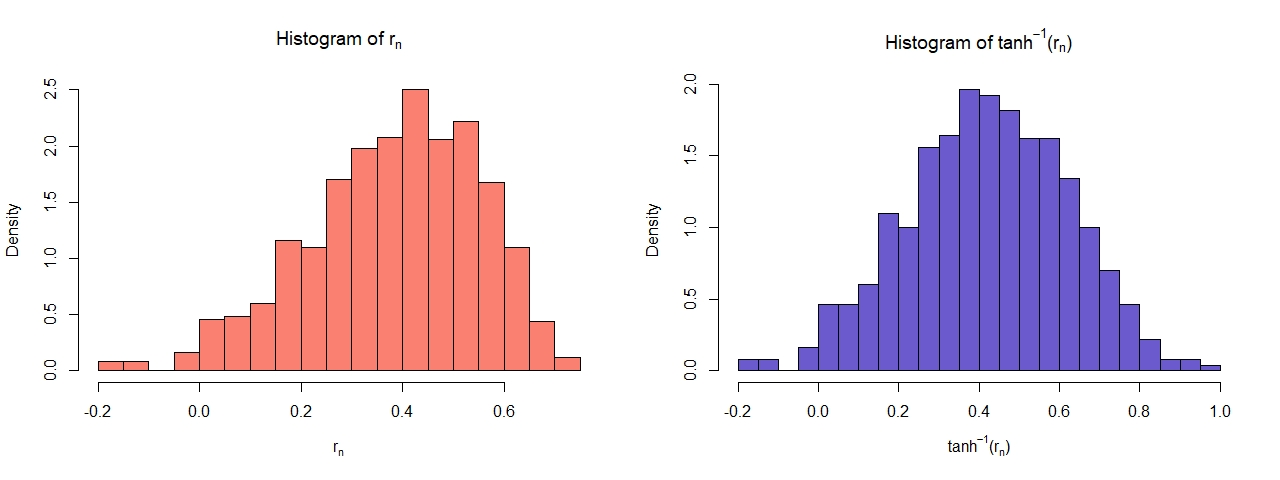
\includegraphics[width = \linewidth]{plot.jpeg}
        \caption{Histogram (density based, not frequency based) of sample correlation coefficent and its transformation}
        \label{fig:6-1}
    \end{figure}

    As it seems from \cref{fig:6-1}, the distribution of sample correlation coefficient $r_n$ is more positively skewed,  while the distribution of the transformed sample correlation coefficent $\tanh^{-1}(r_n)$ is more symmetric in nature, thus resembling the normal distribution better than the untransformed one.
    \end{enumerate}

\end{answer}


\pagebreak
\section{Problem 7}

\begin{problem}
Let $X_1,X_2,\cdots,X_n$ be a random sample from a double exponential distribution with density
$$f(x,\theta)=\dfrac{1}{2}e^{-|x-\theta|},\quad -\infty<x<\infty $$
where $\theta \in \R$ is an unknown location parameter.
\begin{itemize}
    \item[(a)] Find the maximum likelihood estimator (MLE) of $\theta$ and find the asymptotic (non-degenerate) distribution of properly normalized MLE.
    \item[(b)] Find the limiting non-degenerate distribution of the sample
    interquartile range (i.e., the difference between the third and first sample quartiles). 
\end{itemize}
\end{problem}

\begin{answer}
    \begin{enumerate}
        \item[(a)] Note that the likelihood function is given by;
        
        $$\mathcal{L}_n(\theta; X_1, X_2, \dots X_n) = \prod_{i=1}^{n} f(X_i, \theta) = \dfrac{1}{2^n} e^{-\sum_{i=1}^{n} \vert X_i - \theta \vert }$$

        Therefore, to maximize the likelihood $\mathcal{L}_n$, is same as maximizing the log-likelihood $\ell_n = \log\mathcal{L}_n = -n \log 2 - \sum_{i=1}^{n} \vert X_i - \theta \vert$, i.e. same as minimizing $\sum_{i=1}^{n} \vert X_i - \theta \vert$. It is known that, this minimization happens if $\widehat{\theta_n} = X_M$, the sample median\footnote{This is true as one can group observations together like $\sum_{k=1}^{[n/2]} \vert X_{(k)} - \theta \vert + \vert X_{(n-k)} - \theta \vert$ and for each such pair the sum is minimum if $\theta \in (X_{(k)}, X_{(n-k)})$ by triangle inequality}.

        Specifically, the minimization does not lead to a unique minima in case when $n$ is even. In that case, any value between $X_{(\left[ n/2\right])}$ and $X_{(\left[ (n+1)/2\right])}$ is MLE, where $X_{(k)}$ is the $k$-th order statistic.

        Now, to find the asymptotic non-degenerate distribution of properly normalized MLE, we use the result on asymptotic distribution of sample quantile along with Representation theorem.

        Let us choose, $p_n \in (0, 1)$ such that, $\left[ \dfrac{n}{2} \right]/n \leq p_n \leq \left[ \dfrac{n+1}{2} \right]/n$. Let, $p = 1/2$. Then, $\vert p_n - p\vert \leq \dfrac{1}{n} = O(n^{-1/2})$. Let, $X'_{p_n}$ be the $p_n$-th sample quantile. Here, the distribution function $F$ is continuous, differentiable and has a density $f(x, \theta)$ as specified in the question. Also note that, 

        $$
        \int_{-\infty}^{\theta}f(x, \theta) = \dfrac{1}{2} \int_{-\infty}^{\theta} e^{-\vert x - \theta \vert} dx = \dfrac{1}{2} \int_{-\infty}^{0} e^{-z}dz = \dfrac{1}{2}
        $$

        Thus, the population median is $\xi_{1/2} = \theta$. Finally, at $x = \xi_{1/2}$, the density takes value $f(\xi_{1/2}, \theta) = \dfrac{1}{2}e^{-\vert \theta - \theta \vert} = \dfrac{1}{2}$, which is positive. 

        Therefore, by the result on asymptotic distribution of sample quantile if follows that;

        \begin{equation}
            \sqrt{n} (X'_{p_n} - a_n) \xrightarrow{d} \normal\left( 0, \dfrac{1/4}{f(\xi_{1/2})^2}\right) \equiv \normal\left( 0, 1\right)
            \label{eqn:7-1}            
        \end{equation}

        where $a_n = \xi_{1/2} + \dfrac{(p_n - 1/2)}{f(\xi_{1/2})}$. However, $a_n = \theta + 2\left[ (p_n - 1/2) \right] \rightarrow \theta$, as $\vert p_n - 1/2 \vert \leq 1/n \rightarrow 0$ with $n\rightarrow \infty$. Therefore, by an application of Polya's theorem, it follows from \cref{eqn:7-1} that, 

        \begin{equation}
            \sqrt{n} (X'_{p_n} - \theta) \xrightarrow{d} \normal\left( 0, 1\right)
            \label{eqn:7-2}
        \end{equation}

        Since it holds for any $p_n$ satisfying $\left[ \dfrac{n}{2} \right]/n \leq p_n \leq \left[ \dfrac{n+1}{2} \right]/n$, it holds for any MLE. Thus, the properly normalized MLE $\sqrt{n}(\widehat{\theta_n} - \theta)$ is asymptotically normally distributed with mean 0 and variance 1.

        This completes the first part.

        \item[(b)] Let us first obtain the population first and third quantiles, denoted by $\xi_1$ and $\xi_3$ respectively.
        
        Considering $\int_{-\infty}^{\xi_1} f(x, \theta) dx = 1/4$ yields, 

        \begin{align*}
            & \int_{-\infty}^{\xi_1} \dfrac{1}{2} e^{-\vert x - \theta \vert}dx = \dfrac{1}{4}\\
            \Rightarrow \quad & \int_{-\infty}^{(\xi_1 - \theta)} e^{-\vert z \vert} dz = \dfrac{1}{2} \quad \text{with } z = (x - \theta)\\
            \Rightarrow \quad & e^{\xi_1 - \theta} = 1/2\\
            \Rightarrow \quad & \xi_1 = \theta - \log 2\\
        \end{align*}

        Since the given distribution is symmetric with respect to location parameter $\theta$, $\xi_3 = \theta + \log 2$. Note that,

        $$
        f(\xi_1, \theta) = f(\xi_3, \theta) = \dfrac{1}{2} e^{-\vert \log 2\vert} = \dfrac{1}{2} e^{\log (1/2)} = \dfrac{1}{4}
        $$
        
        By using multivariate CLT and Representation theorem, we have the following result.

        Let, $0 < p_1 < p_2 < \dots < p_k$ and let $p_{in} = p_i + O\left( n^{-1/2} \right)$, with $F'(\xi_{p_i}) > 0 \quad \forall i$, where $\xi_{p}$ is the $p$-th quantile of the distribution function $F$. Then, 

        $$U_n = \left( \sqrt{n}(Y_{p_{1n}, n} - a_{1n}), \sqrt{n}(Y_{p_{2n}, n} - a_{2n}), \dots \sqrt{n}(Y_{p_{kn}, n} - a_{kn})  \right)$$

        is asymptotically normal with mean vector $0$ and dispersion matrix $\Sigma = ((\sigma_{ij}))_{i, j = 1}^{k}$ where $\sigma_{ij} = \sigma_{ji} = \dfrac{p_i(1 - p_j)}{F'(\xi_{p_i}) F'(\xi_{p_j})}$ for $i \leq j$, where $Y_{p, n}$ is the sample $p$-th quantile based on a sample of size $n$.

        Using this result for $p_1 = 1/4$ and $p_2 = 3/4$ only, and denoting the first sample quartile as $Q_{1, n}$ and the third sample quartile as $Q_{3, n}$, we get that,  

        \begin{equation}
            \sqrt{n}\left(
            \begin{bmatrix}
                Q_{1, n}\\
                Q_{3, n} 
            \end{bmatrix}
            - \begin{bmatrix}
                \xi_1\\
                \xi_3\\
            \end{bmatrix}
            \right) \xrightarrow{d}
            \mathcal{MVN} \left( \bm{0}_2, \Sigma \right)
        \label{eqn:7-3}
        \end{equation}

        where,

        \begin{align*}
            \Sigma
            & = \begin{bmatrix}
                \dfrac{1/4 \times 3/4}{f(\xi_1)^2} & \dfrac{(1/4)^2}{f(\xi_1)f(\xi_3)}\\
                & \\
                \dfrac{(1/4)^2}{f(\xi_1)f(\xi_3)} & \dfrac{3/4 \times 1/4}{f(\xi_3)^2}\\
            \end{bmatrix}\\
            & \\
            & = \begin{bmatrix}
                (3/16)/(1/16) & (1/16)/(1/16)\\
                (1/16)/(1/16) & (3/16)/(1/16)\\
            \end{bmatrix}\\
            & \\
            & = \begin{bmatrix}
                3 & 1\\
                1 & 3\\
            \end{bmatrix}
        \end{align*}
        
        Now, consider the function $g(x, y) = (y - x)$, with $g: \R^2 \rightarrow \R$ being a differentiable function. Note that, $g\left( \begin{bmatrix}
            Q_{1, n}\\ Q_{3, n}
        \end{bmatrix} \right) = Q_{3, n} - Q_{1, n}$, the sample interquartile range, while $g\left( \begin{bmatrix}
            \xi_1 \\ \xi_3
        \end{bmatrix}\right) = \xi_3 - \xi_1 = 2 \log 2 = \log 4$. Thus an application of multivariate delta method to \cref{eqn:7-3} yields;

        \begin{equation}
            \sqrt{n} ((Q_{3, n} - Q_{1, n}) - \log 4) \xrightarrow{d} \normal\left( 0, (\nabla g(\xi_1, \xi_3))^{\intercal} \Sigma (\nabla g(\xi_1, \xi_3))  \right)
            \label{eqn:7-4}
        \end{equation}

        With $g(x, y) = (y - x)$, $\nabla g(x, y) = (-1, 1)^{\intercal}$ for any $x, y \in \R$. Therefore, 
        $$(\nabla g(\xi_1, \xi_3))^{\intercal} \Sigma (\nabla g(\xi_1, \xi_3)) = (3 - 2 + 3) = 4$$
        Finally denoting $(Q_{3,n} - Q_{1, n}) = IQR_n$ we obtain from \cref{eqn:7-4} that,

        $$
        \sqrt{n}(IQR_n - \log 4) \xrightarrow{d} \normal(0, 4)
        $$

        This completes part (b).
    \end{enumerate}
\end{answer}


\pagebreak
\section{Problem 8}

\begin{problem}
Let $X_1,X_2,\cdots,X_n$ be a random sample from $\mathcal{N}(\theta,1)$. Find the joint asymptotic distribution of suitably normalized sample mean and sample median.
\end{problem}

\begin{answer}
    Let, $\bar{X}_n = \dfrac{1}{n} \sum_{i=1}^{n}X_i$, be the sample mean. Since, $X_i \sim \normal(\theta, 1)$, hence $\bar{X}_n \sim \normal(\theta, 1/n)$.

    Let us denote the sample median of $X_i$'s based on as $X_{Me, n}$.

    Also, $\bar{X}_n$ is a minimal sufficent statistic for $\theta$, while $Y_i = (X_i - \bar{X}_n)$ are ancillary for $\theta$, in case of normal distribution. Thus, by Basu's theorem, it follows that $\bar{X}_n$ is independent of $Y_i$'s. Thus, $\bar{X}_n$ is also independent of the median of $Y_i$'s, say $Y_{Me, n}$. However, the sample median of $X_i$'s is simply $X_{Me, n} = Y_{Me, n} + \bar{X}_n$.

    Therefore, we shall proceed by finding the joint asymptotic distribution of $\bar{X}_n$ and $Y_{Me, n}$ first. Since, $Y_i$'s are not independent of each other, it is not possible to obtain the asymptotic distribution of sample median of $Y_i$'s simply by direct use of the theorem regarding asymptotic distribution of sample quantiles.


    We shall use \textbf{Levy's Continuity Theorem}\footnote{\textbf{Statement of the theorem:} A sequence of random variables $X_n$ converges in distribution to the random variable $X$ if and only if the sequence of its characteristic function $\psi_{X_n}(t)$ converges pointwise to a function $\psi(t)$ which is continuous at $t = 0$, and in that case $\psi$ is the characteristic function of $X$} to find this joint asymptotic distribution. 

    Note that, by the result on asymptotic distribution of sample median, it follows that $\sqrt{n}(X_{Me, n} - \theta)$ is asymptotically normally distributed with mean $0$ and variance $\dfrac{1/4}{\phi(\theta)^2}$, where $\phi(\cdot)$ is the density function of the normal distribution with mean $\theta$ and variance $1$. Clearly, $\phi(\theta) = \dfrac{1}{\sqrt{2\pi}}$. Thus we have,
    
    \begin{equation}
        \sqrt{n}(X_{Me, n} - \theta) \xrightarrow{d} \normal\left( 0, \dfrac{1/4}{1/2\pi} \right) \equiv \normal\left( 0, \dfrac{\pi}{2} \right)
        \label{eqn:8-1}
    \end{equation}

    It is known that the characteristic function of a random variable normally distributed with mean $\theta$ and variance $\sigma^2$ is given as $\exp\left[ i\mu t - \dfrac{\sigma^2t^2}{2} \right]$. Therefore, it follows by Levy's Continuity Theorem,
    
    \begin{equation}
        \lim_{n \rightarrow \infty} \psi_{\sqrt{n}(X_{Me, n} - \theta)}(t) = e^{-\frac{\pi}{4}t^2}
        \label{eqn:8-2}        
    \end{equation}

    On the other hand, $\sqrt{n}(X_{Me, n} - \theta) = \sqrt{n} (\bar{X}_n - \theta) + \sqrt{n}Y_{Me, n}$ and as noted above, these two quantities are independent. Thus, $\psi_{\sqrt{n}(X_{Me, n} - \theta)}(t) = \psi_{\sqrt{n}(\bar{X}_n - \theta)}(t) \times \psi_{\sqrt{n}Y_{Me, n}}(t)$ for any $t \in \R$. Since, $\sqrt{n} (\bar{X}_n - \theta) \sim \normal(0, 1)$, it follows that $\psi_{\sqrt{n}(\bar{X}_n - \theta)}(t) = e^{-t^2/2}$. Therefore,

    \begin{align*}
        \lim_{n \rightarrow \infty} \psi_{\sqrt{n}Y_{Me, n}}(t)
        & = \lim_{n \rightarrow \infty} \dfrac{\psi_{\sqrt{n}(X_{Me, n} - \theta)}(t) }{\psi_{\sqrt{n} (\bar{X}_n - \theta)}(t)}\\
        & = \dfrac{\lim_{n \rightarrow \infty}  \psi_{\sqrt{n}(X_{Me, n} - \theta)}(t) }{e^{-t^2/2}} \qquad \text{, since the individual limit exists}\\ 
        & \qquad \qquad \qquad \qquad \qquad \qquad \qquad \text{ and denominator is nonzero}\\
        & = e^{-t^2(\frac{\pi}{2} - 1)/2}
    \end{align*}

    Clearly, this is the characteristic function of a normally distributed random variable with mean $0$ and variance $\left( \dfrac{\pi}{2} - 1 \right)$, and this is continuous at $t = 0$. Hence, by application of Levy's Continuity theorem, it follows that;
    
    \begin{equation*}
        \sqrt{n}Y_{Me, n} \xrightarrow{d} \normal\left( 0, \left( \dfrac{\pi}{2} - 1 \right) \right)
    \end{equation*}

    Now since $\bar{X}_n$ is independent of $Y_{Me, n}$, hence any linear combination, namely for any $a, b \in \R$, we have,

    \begin{equation}
        a \sqrt{n}(\bar{X}_n - \theta) + b \sqrt{n} Y_{Me, n} \xrightarrow{d} \normal\left( 0, a + b\left(\dfrac{\pi}{2} - 1\right) \right)
        \label{eqn:8-3}
    \end{equation}

    Thus applying Cramer Wold theorem to \cref{eqn:8-3}, we obtain the required joint asymptotic distribution as;

    \begin{equation}
        \sqrt{n} \left(
            \begin{bmatrix}
                \bar{X}_n\\ Y_{Me, n}
            \end{bmatrix} - \begin{bmatrix}
                \theta \\ 0
            \end{bmatrix}
        \right) \xrightarrow{d} \mathcal{MVN}\left( \bm{0}_2, \begin{bmatrix}
            1 & 0\\
            0 & \left(\pi/2 - 1\right)
        \end{bmatrix} \right)
        \label{eqn:8-4}
    \end{equation}

    Now, consider the function $g: \R^2 \rightarrow \R^2$ such that $g(x, y) = (x, x+y)$. Then, the jacobian of the function is $J_g(x, y) = \begin{bmatrix}
        1 & 1\\
        0 & 1\\
    \end{bmatrix}$. Also, $g(\bar{X}_n, Y_{Me,n}) = (\bar{X}_n, \bar{X}_n + Y_{Me, n}) = (\bar{X}_n, X_{Me, n})$, and $g(\theta, 0) = (\theta, \theta)$.

    Therefore, by an application of multivariate delta method to \cref{eqn:8-4}, it follows that;

    $$
    \sqrt{n} \left(
        \begin{bmatrix}
            \bar{X}_n\\ X_{Me, n}
        \end{bmatrix} - \begin{bmatrix}
            \theta \\ \theta
        \end{bmatrix}
    \right) \xrightarrow{d} \mathcal{MVN}\left( \bm{0}_2, J_g(\theta, 0)^{\intercal} \begin{bmatrix}
        1 & 0\\
        0 & \left(\pi/2 - 1\right)
    \end{bmatrix} J_g(\theta, 0) \right)
    $$

    Note that,

    \begin{align*}
        J_g(\theta, 0)^{\intercal} \begin{bmatrix}
            1 & 0\\
            0 & \left(\pi/2 - 1\right)
        \end{bmatrix} J_g(\theta, 0)
        & = \begin{bmatrix}
            1 & 0\\
            1 & 1
        \end{bmatrix}
        \begin{bmatrix}
            1 & 0\\
            0 & \left(\pi/2 - 1\right)
        \end{bmatrix}
        \begin{bmatrix}
            1 & 1\\
            0 & 1
        \end{bmatrix}
        & \\
        & = \begin{bmatrix}
            1 & 0\\
            1 & \left(\pi/2 - 1\right)\\
        \end{bmatrix} \begin{bmatrix}
            1 & 1\\
            0 & 1\\
        \end{bmatrix}
        & = \begin{bmatrix}
            1 & 1\\
            1 & \pi/2
        \end{bmatrix}
    \end{align*}

    Therefore, a suiatably transformed and scaled joint asymptotic distribution of sample mean and sample median is given by,

    \begin{equation*}
        \sqrt{n} \left(
        \begin{bmatrix}
            \bar{X}_n\\ X_{Me, n}
        \end{bmatrix} - \begin{bmatrix}
            \theta \\ \theta
        \end{bmatrix}
    \right) \xrightarrow{d} \mathcal{MVN}_2\left( \bm{0}_2,
    \begin{bmatrix}
        1 & 1\\
        1 & \pi/2
    \end{bmatrix}
    \right)
    \end{equation*}


\end{answer}

\pagebreak
\section{Problem 9}

\begin{problem}
Let $X_1,X_2,\cdots,X_n$ be a random sample from $\mathcal{N}(\theta,1)$ where $\theta$ is an unknown integer. Find the maximum likelihood estimator (MLE) $\hat{\theta}_n$ of $\theta$. Prove that it is not possible to find a sequence of real constants $a_n$ such that $a_n\left(\hat{\theta}_n-\theta\right)$ converges to a non-degenerate limit distribution.
\end{problem}

\begin{answer}
    
    We start by writing the likelihood function,

    $$
    \mathcal{L}(\theta) = \dfrac{1}{(2\pi)^{(n/2)}} \exp\left[ -\dfrac{1}{2} \sum_{i=1}^{n} (X_i - \theta)^2 \right] \bm{1}_{ \{\theta \in \Z\} }
    $$

    where $\bm{1}_{A}$ is the indicator function of the set $A$ and $\Z$ is the set of integers. Note that, the likelihood can be expressed as,

    $$
    \mathcal{L}(\theta) = \dfrac{1}{(2\pi)^{(n/2)}} \exp\left[ -\dfrac{1}{2} \sum_{i=1}^{n} (X_i - \bar{X}_n)^2 - \dfrac{n}{2} (\bar{X}_n - \theta)^2 \right] \bm{1}_{ \{\theta \in \Z\} }
    $$
    
    The likelihood function takes nonzero value if and only if $\theta \in \Z$ and is decreasing in the magnitude of $\vert \bar{X}_n - \theta \vert$ restricted to $\theta \in \Z$. Thus, the MLE of $\theta$ would be equal to the nearest integer of $\bar{X}_n$, i.e.

    $$
    \widehat{\theta}_n = \begin{cases}
        \lceil \bar{X}_n \rceil & \text{ if } \{ \bar{X}_n \} > 1/2\\
        \lfloor \bar{X}_n \rfloor & \text{ if } \{ \bar{X}_n \} \leq 1/2\\
    \end{cases}
    $$

    where $\lceil \cdot \rceil$ is the ceiling function, $\lfloor \cdot \rfloor$ is the floor function and $\{ x\}$ is the fractional part of $x$. In other words, $\widehat{\theta}_n$ is the unique integer in the interval $[\bar{X}_n - 1/2, \bar{X}_n + 1/2)$.

    Now let us consider the probability under $\theta$ that the MLE is not same as the true $\theta \in \Z$, 

    \begin{align*}
        \prob_{\theta}(\widehat{\theta}_n \neq \theta)
        & = \prob_{\theta}\left( \text{Closest integer to } \bar{X}_n \neq \theta \right)\\
        & = \prob_{\theta} \left( \theta \notin [\bar{X}_n - 1/2, \bar{X}_n + 1/2) \right)\\
        & = \prob_{\theta} \left( \{ \bar{X}_n > \theta + 1/2 \} \cup \{ \bar{X}_n \leq \theta - 1/2 \}\right)\\
        & = \prob_{\theta} (\bar{X}_n > \theta + 1/2) + \prob_{\theta} (\bar{X}_n \leq \theta - 1/2), \text{ as two events are disjoint}\\
        & = 2 \prob_{\theta} (\sqrt{n}(\bar{X}_n - \theta) > \sqrt{n}/2 )\\
        & = 2 \left( 1 - \Phi(\sqrt{n}/2) \right), \qquad \text{ since } \sqrt{n}(\bar{X}_n - \theta) \sim \normal(0, 1)
    \end{align*}

    where $\Phi(\cdot)$ is the cumulative distribution function of a standard normal random variable.

    Now, we shall prove a tail bound for this probability. Let, $Z$ be a standard normal random variable and $\phi(\cdot)$ be the density function for standard normal distribution. Then, for $t > 0$,

    \begin{align*}
        \E(e^{t(Z - a)}) & = \int_{-\infty}^{\infty} e^{t(z - a)} \phi(z)dz\\
        & \geq \int_{a}^{\infty} e^{t(z - a)} \phi(z)dz\\
        & \geq \int_{a}^{\infty} \phi(z)dz \text{, since } e^{t(z-a)} \geq 1 \text{ for } z \geq a, t > 0\\
        & = (1 - \Phi(a))
    \end{align*}

    Therefore, 

    $$
    (1 - \Phi(a)) \leq \inf_{t > 0} \E(e^{t(Z - a)}) = \inf_{t > 0} e^{-at} \E(e^{tZ}) = \inf_{t > 0} e^{-at} M_Z(t)
    $$

    where $M_Z(t)$ is the moment generating function for $Z$. However, it is known that for standard normal distribution, the moment generating function $M_Z(t) = e^{t^2/2}$. Thus, it follows that;


    \begin{equation}
        (1 - \Phi(a)) \leq \inf_{t > 0} e^{t^2/2 - at} = e^{-a^2/2}
        \label{eqn:9-1}        
    \end{equation}

    with the infimum being achieved at $t = a$. Therefore, applying \cref{eqn:9-1} as a tail bound, we obtain that;

    \begin{equation}
        \prob_{\theta}(\widehat{\theta}_n \neq \theta) \leq 2 \exp\left[ - \dfrac{(\sqrt{n}/2)^2}{2} \right] = 2 \exp\left[ - \dfrac{n^2}{8} \right]
        \label{eqn:9-2}
    \end{equation}

    Hence, it follows from \cref{eqn:9-2},

    \begin{align*}
        \sum_{n=1}^{\infty} \prob_{\theta}(\widehat{\theta} \neq \theta)
        & \leq \sum_{n=1}^{\infty} 2 \exp\left[ - \dfrac{n^2}{8} \right]\\
        & \leq 2 \sum_{n=1}^{\infty} \exp\left[ - \dfrac{n}{8} \right] \qquad \text{as, } e^{-n^2/8} \geq e^{-n/8} \quad \forall n \geq 1\\
        & = 2 \sum_{n=1}^{\infty} \left(e^{-1/8}\right)^n\\
        & = 2 \dfrac{e^{-1/8}}{1 - e^{-1/8}} < \infty \qquad \text{ as } e^{-1/8} < 1
    \end{align*}

    Therefore, by Borel Cantelli Lemma, the event has $\widehat{\theta}_n \neq \theta$ happens infinitely many often has probability equal to 0. In other words, the event $\widehat{\theta}_n = \theta$ happens almost surely after some finite time i.e. for all $n \geq N$ for some large $N$. This essentially means, for all $n \geq N$, 

    $$
    \prob_\theta\left(a_n(\widehat{\theta}_n - \theta) = 0\right)
    \leq \prob_{\theta} \left( (\widehat{\theta}_n - \theta) = 0 \right)
    = 1
    $$

    i.e. it is not possible to find a sequence of real constants $a_n$ such that $a_n(\widehat{\theta}_n - \theta)$ converges to a non-degenerate limit distribution.
\end{answer}

\pagebreak
\section{Problem 10}

\begin{problem}
Let $X_1,X_2,\cdots,X_n$ be i.i.d. with a common density $f(x,\theta)$, where $\theta \in \Theta$ and $\Theta$ consists of only finitely many real numbers. Assume also that the set $\{x : f(x, \theta) > 0\}$ is the same for all $\theta \in \Theta$ and that the distributions under different $\theta$’s are different. If $\theta_0$ is the true value of $\theta$, prove that with
probability tending to one (under $\theta_0$) as $n\rightarrow\infty$, the likelihood function will be maximized at the value $\theta = \theta_0$.
\end{problem}

\begin{answer}
    We are given that $X_1,X_2,\cdots,X_n$ be i.i.d. with a common density $f(x,\theta)$, where $\theta \in \Theta$ and $\Theta$ consists of only finitely many real numbers. Let us assume, $\Theta = \left\{ \theta_0, \theta_1, \dots \theta_k \right\}$ among which $\theta_0$ is the true parameter.

    We start by considering the likelihood ratio,

    \begin{align*}
        LR(\theta, \theta_0) & =  \dfrac{\mathcal{L}(\theta; X_1, X_2, \dots X_n)}{\mathcal{L}(\theta_0; X_1, X_2, \dots X_n)}\\
        & = \dfrac{\prod_{i=1}^{n} f(X_i, \theta)}{\prod_{i=1}^{n} f(X_i, \theta_0)}\\
        & = \prod_{i=1}^{n} \dfrac{f(X_i, \theta)}{f(X_i, \theta_0)}\\
        \Rightarrow \quad \log LR(\theta, \theta_0) & = \sum_{i = 1}^{n} \log \left(\dfrac{f(X_i, \theta)}{f(X_i, \theta_0)} \right)\\
    \end{align*}

    Since, the set $A = \{ x: f(x, \theta) > 0 \}$ is same for all $\theta \in \Theta$, and the ratios $f(x, \theta)/f(x, \theta_0)$ and its logarithm make sense for any $x \in A$, the above individual logarithms make sense as $X_i \in A$ for all $i = 1, 2, \dots n$.

    Now, since $X_i$'s are i.i.d., so is the ratio $f(X_i, \theta)/f(X_i, \theta_0)$ and its natural logarithm. Hence, by Weak Law of Large Numbers,

    $$
    \dfrac{1}{n} \sum_{i = 1}^{n} \log \left(\dfrac{f(X_i, \theta)}{f(X_i, \theta_0)} \right) \xrightarrow{P} \E_{\theta_0} \left( \log \left(\dfrac{f(X_1, \theta)}{f(X_1, \theta_0)} \right) \right) \qquad \text{as, } \theta_0 \text{ is assumed to be true parameter}
    $$

    Now, by Jensen's inequality,

    \begin{align*}
        \E_{\theta_0} \left[ \log \left(\dfrac{f(X_1, \theta)}{f(X_1, \theta_0)} \right) \right]
        & \leq \log \left( \E_{\theta_0} \left[ \dfrac{f(X_1, \theta)}{f(X_1, \theta_0)} \right] \right)\\
        & = \log \left( \int_{x \in A} \dfrac{f(x, \theta)}{f(x, \theta_0)} f(x, \theta_0)dx \right)\\
        & = \log 1 \quad \text{since, for } x\in A, f(x, \theta_0) \neq 0\\
        & = 0
    \end{align*}

    with equality if and only if $f(x, \theta_0) = f(x, \theta)$ for all $x \in A$, where $A$ is the common support of both of these distributions. However, as the distributions under different $\theta$'s are different (i.e. identifiability condition), this yields that in the above inequality, equality will hold if and only if $\theta = \theta_0$.

    Thus, for any $\theta \neq \theta_0$,

    \begin{align*}
        & \prob_{\theta_0} \left( \dfrac{1}{n}\log LR(\theta, \theta_0) < 0 \right) \rightarrow 1\\
        \Rightarrow \quad & \prob_{\theta_0} \left( LR(\theta, \theta_0) < 1 \right) \rightarrow 1\\
        \Rightarrow \quad & \prob_{\theta_0} \left( \mathcal{L}_n(\theta) < \mathcal{L}_n(\theta_0) \right) \rightarrow 1 \qquad \text{where, } \mathcal{L}_n(\theta) = \mathcal{L}(\theta; X_1, X_2, \dots X_n)\\
        \Rightarrow \quad & \prob_{\theta_0} \left( \mathcal{L}_n(\theta) \geq \mathcal{L}_n(\theta_0) \right) \rightarrow 0
    \end{align*}

    Therefore, for a given $\epsilon > 0$, for $\theta_i$, $i = 1, 2, \dots k$, there exists $N_i$ such that for all $n \geq N_i$, 

    \begin{equation}
        \prob_{\theta_0}(\mathcal{L}_n(\theta_i) \geq \mathcal{L}_n(\theta_0)) < \dfrac{\epsilon}{k}
        \label{eqn:10-1}        
    \end{equation}

    Hence, for all $n \geq N = \max\{ N_1, N_2, \dots N_k \}$ we must have;

    \begin{align*}
        \prob_{\theta_0} \left( \text{Likelihood is maximized at } \theta = \theta_0 \right)
        & = \prob_{\theta_0} \left( \mathcal{L}_n(\theta_0) > \mathcal{L}_n(\theta_i); \forall i = 1, 2, \dots k \right)\\
        & = \prob_{\theta_0} \left( \cap_{i=1}^{k} \{ \mathcal{L}_n(\theta_0) > \mathcal{L}_n(\theta_i)\} \right)\\
        & = 1 - \prob_{\theta_0} \left( \cup_{i=1}^{k} \{ \mathcal{L}_n(\theta_0) \leq \mathcal{L}_n(\theta_i)\} \right)\\
        & \geq 1 - \sum_{i = 1}^{k} \prob_{\theta_0} \left( \mathcal{L}_n(\theta_0) \leq \mathcal{L}_n(\theta_i) \right)\\
        & \geq 1 - \sum_{i=1}^{k} \epsilon/k \qquad \text{by \cref{eqn:10-1}}\\
        & = (1 - \epsilon)
    \end{align*}

    Therefore, $\prob_{\theta_0} \left( \text{Likelihood is maximized at } \theta = \theta_0 \right) \rightarrow 1$ as $n \rightarrow \infty$.

\end{answer}

\pagebreak
\section{Problem 11}

\begin{problem}
Let $X_1,X_2,\cdots,X_n$ be i.i.d. with a common density $f(x,\theta)$ given by,
$$f(x,\theta) = \dfrac{e^{-(x-\theta)}}{\left[ 1+e^{-(x-\theta)} \right]^2}, \quad -\infty<x<\infty,$$
where $\theta \in \R$ is unknown. Assume that Conditions (A1)–(A7) of the section
on MLE hold.
\begin{itemize}
    \item[(a)] Does there exist a consistent maximum likelihood estimator of $\theta$ for this problem? Justify your answer.
     \item[(b)] Can you suggest any sequence of functions $g_n(\cdot)$ (depending on $n$) of $\Bar{X}_n$ such that $g_n(\Bar{X}_n)$ (after suitable centering and scaling) converges in distribution to $\normal\left(0,\dfrac{1}{I(\theta)}\right)$ where $I(\theta)$ is the Fisher Information? Justify your answer. 
\end{itemize}
\end{problem}

\begin{answer}
    
    \begin{enumerate}
        \item[(a)] We start by considering the likelihood;
        
        $$
        \mathcal{L}_n(\theta) = \prod_{i=1}^{n} f(X_i, \theta) = \prod_{i=1}^{n} \dfrac{e^{-(X_i - \theta)}}{\left[ 1 + e^{-(X_i - \theta)} \right]^2}
        $$

        Therefore, the log-likelihood is;

        $$
        \log\mathcal{L}_n(\theta) = \ell_n(\theta) = \sum_{i=1}^{n} (\theta - X_i) - 2\log\left[ 1 + e^{-(X_i - \theta)} \right]
        $$

        Since the log-likelihood is a continuous function of $\theta$ for all $\theta \in \R$, the maximum likelihood estimator can be easily obtained by setting the derivative of the log-likelihood equal to 0, thus considering a likelihood equation.

        \begin{align*}
            \dfrac{d\ell_n}{d\theta} = 0
            \implies \quad & n - 2 \sum_{i=1}^{n} \dfrac{e^{-(X_i - \theta)}}{1 + e^{-(X_i - \theta)}} = 0\\
            \implies \quad & n - 2 \sum_{i = 1}^{n} \left[ 1 - \dfrac{1}{1 + e^{-(X_i - \theta)}} \right] = 0\\
            \implies \quad & n - 2n + 2\sum_{i=1}^{n} \dfrac{1}{1 + e^{-(X_i - \theta)}} = 0\\
            \implies \quad & \sum_{i=1}^{n} \dfrac{1}{1 + e^{-(X_i - \theta)}} = \dfrac{n}{2}\\
        \end{align*}

        In the last equation, the left hand side is sum of functions of type $1/(1 + e^{-(x - \theta)})$, which is a strictly decreasing, continuous function in $\theta$. Also, as $\theta \rightarrow \infty$, $1/(1 + e^{-(x - \theta)}) \rightarrow 0$ for any $x \in \R$, thus the left hand side goes to $0$. On the other hand, as $\theta \rightarrow (-\infty)$, $1/(1 + e^{-(x - \theta)}) \rightarrow 1$ for any $x \in \R$, thus the left hand side goes to $n$. Therefore, for any $n \in \N$, the left hand side strictly decreases continuously from $n$ to $0$ as $\theta$ moves from $(-\infty)$ to $\infty$, showing that there must exists a unique $\widehat{\theta}_n$ such that the above equation holds, i.e. there must exist a unique solution to the likelihood equation.

        Clearly, this unique solution must be the unique MLE for the given setup. Now, since assumptions (A1)-(A3) hold, by theorem 9.1 of the notes it follows that, for any $\delta > 0$, where the true parameter is $\theta_0$,

        \begin{equation}
            \prob_{\theta_0} \left[ \dfrac{\partial\log \mathcal{L}_n}{\partial \theta} = 0 \text{ has a solution in } (\theta_0 - \delta, \theta_0 + \delta) \right] \rightarrow 1
            \label{eqn:11-1}  
        \end{equation}

        However, since the solution to the likelihood equation is found to be unique, it must correspond to $\widehat{\theta}_n$. Therefore, by \cref{eqn:11-1} it follows that for any $\delta > 0$,

        $$
        \prob_{\theta_0} \left[ \vert \widehat{\theta}_n - \theta_0 \vert < \delta \right] \rightarrow 1
        $$

        i.e.

        $$
        \prob_{\theta_0} \left[ \vert \widehat{\theta}_n - \theta_0 \vert \geq \delta \right] \rightarrow 0
        $$

        This shows that the MLE is consistent in this case, i.e. $\widehat{\theta}_n \xrightarrow{P} \theta$.

        \item[(b)] Starting from the quantity $\dfrac{d \ell_n}{d \theta}$, we have;
        
        $$
        \dfrac{d^2 \ell_n}{d \theta^2} 
        = -2 \sum_{i=1}^{n} \dfrac{d}{d\theta} \left[1 - \dfrac{1}{(1 + e^{-(X_i - \theta)})} \right]\\
        = -2 \sum_{i=1}^{n} \dfrac{e^{-(X_i - \theta)}}{(1 + e^{-(X_i - \theta)})^2}
        $$

        Therefore,

        \begin{align*}
            \mathcal{I}_n(\theta)
            & = \E\left[ -\dfrac{d^2 \ell_n}{d \theta^2} \right]\\
            & = 2n \E\left[ \dfrac{e^{-(X_1 - \theta)}}{(1 + e^{-(X_1 - \theta)})^2} \right] \qquad \text{ since } X_i\text{'s are i.i.d.}\\
            & = 2n \int_{-\infty}^{\infty} \dfrac{e^{-2(x-\theta)}}{(1 + e^{-(x - \theta)})^4} dx
        \end{align*}

        Substituting $z = (1 + e^{-(x-\theta)})$ yields,

        \begin{align*}
            \mathcal{I}_n(\theta)
            & = 2n \int_{1}^{\infty} \dfrac{(z - 1)}{z^4} dz
            & = 2n \left[ \int_{1}^{\infty} z^{-3}dz - \int_{1}^{\infty} z^{-4}dz \right]\\
            & = 2n \left[ \dfrac{1}{2} - \dfrac{1}{3} \right]\\
            & = 2n \times \dfrac{1}{6} = \dfrac{n}{3}
        \end{align*}

        which is independent of $\theta$. In other words, $\mathcal{I}(\theta) = 1/3$, for a single sample from the distribution.

        Now, we know that as $X_i$ has the same density function as a logisitic distribution with location parameter $\theta$ and scale parameter $1$, it follows that $\E(X_i) = \theta$ and $\Var(X_i) = \pi^2/3$. Therefore, by Central Limit theorem, it follows that

        \begin{equation}
            \sqrt{n}\dfrac{(\bar{X}_n - \theta)}{\pi / \sqrt{3}} \xrightarrow{d} \normal(0, 1)
            \label{eqn:11-2}
        \end{equation}

        Thus if we consider, $g : \R \rightarrow \R$ such that $g(x) = \dfrac{3}{\pi} x$, then 

        \begin{equation}
            \sqrt{n}(g(\bar{X}_n) - g(\theta)) \xrightarrow{d} \normal\left(0, \dfrac{\pi^2}{3} \times \dfrac{9}{\pi^2} \right)
            \equiv \normal(0, 3) \equiv \normal\left( 0, 1/\mathcal{I}(\theta) \right)
            \label{eqn:11-3}
        \end{equation}

        Therefore, we can consider the constant sequence of functions, namely $g_n(x) = \dfrac{3}{\pi} x$ such that the sequence of random variables $g_n(\bar{X}_n)$, after suitable centering and scaling as shown in \cref{eqn:11-3}, converges in distribution to $\normal(0, 1/\mathcal{I}(\theta))$.

    \end{enumerate}

\end{answer}

\pagebreak
\section{Problem 12}

\begin{problem}
Let $X_1,X_2,\cdots,X_n$ be i.i.d. with a common density $f(x,\theta)$ given by,
$$f(x,\theta) = e^{-(x-\theta)}\quad x\geq \theta, \quad -\infty<\theta<\infty,$$
\begin{itemize}
    \item[(a)] Find the MLE $\hat{\theta}_n$ of $\theta$ and the limiting non-degenerate distribution of suitably normalized $\left(\hat{\theta}_n-\theta\right)$.
    \item[(b)] Given that $\theta\leq 1$, find the MLE $\Tilde{\theta}_n$ of $\theta$ and also find the limiting non-degenerate distribution of suitably normalized $\left(\Tilde{\theta}_n-\theta\right)$ under $\theta = \theta_0 < 1$. 
\end{itemize}
\end{problem}

\begin{answer}
	\begin{enumerate}
        \item[(a)] The likelihood function is given as follows:
        \begin{align*}
            \mathcal{L}(\theta) 
            & = \prod_{i=1}^{n} f(X_i, \theta)\\
            & = \prod_{i=1}^{n} e^{-(X_i - \theta)} \bm{1}_{\{ X_i \geq \theta\} }\qquad \text{where, } \bm{1}_A \text{ is the indicator function of } A\\
            & = e^{-\sum_{i=1}^{n} (X_i - \theta) } \bm{1}_{ \{X_{(1)} \geq \theta\} }\\
            & = e^{(n\theta - \sum_{i=1}^{n} X_i)} \bm{1}_{ \{X_{(1)} \geq \theta\} }
        \end{align*}
        Now, it is clear that this function takes value $0$ if $\theta > X_{(1)}$, and is monotonically increasing in $\theta$ before $\theta = X_{(1)}$. Hence, the likelihood function is maximized at $\theta = X_{(1)}$.

        Therefore, the MLE is $\widehat{\theta_n} = X_{(1)}$. Now note that,

        \begin{align*}
            \prob_\theta(X_{(1)} > x)
            & = \prod_{i=1}^{n} \prob_\theta(X_i > x) \text{since, the former event is equivalent to the later event}\\
            & = \prod_{i=1}^{n} \int_{x}^{\infty} e^{-(u - \theta)}du\\
            & = \prod_{i=1}^{n} e^{-(x - \theta)}\\
            & = e^{-n(x - \theta)}\\
        \end{align*}

        Therefore,

        \begin{align*}
            \prob_\theta(n(\widehat{\theta_n} - \theta) \leq x)
            & = \prob_\theta(n(X_{(1)} - \theta) \leq x)\\
            & = \prob_\theta\left(X_{(1)} \leq \theta + \dfrac{x}{n}\right)\\
            & = 1 - \prob_\theta\left( X_{(1)} > \theta + \dfrac{x}{n} \right)\\
            & = 1 - \exp\left[ -n\left( \theta + \dfrac{x}{n} - \theta \right)\right] \qquad \text{ by previous derivation}\\
            & = 1 - e^{-x}
        \end{align*}

        which is the cumulative distribution function of exponential distribution with mean $1$. Therefore, the limiting non-degenerate distribution of suitably normalized quantity regarding the MLE is: $n(\widehat{\theta_n} - \theta) \xrightarrow{d} \text{Exp}(1)$, where $\text{Exp}(1)$ is the exponential distribution with scale parameter $1$. 

        \item[(b)] In case it is also given that $\theta \leq 1$, the likelihood function is given by;
        
        $$\mathcal{L}(\theta) = e^{(n\theta - \sum_{i=1}^{n} X_i)} \bm{1}_{ \{X_{(1)} \geq \theta\} } \bm{1}_{ \{ \theta \leq 1 \} }$$

        Therefore, the likelihood function only takes positive value if $\theta \leq \min\{ X_{(1)}, 1\}$ and in the region it takes positive value, the likelihood is monotonically increasing as before. Therefore, the MLE $\widetilde{\theta_n}$ in this case is given by, $\widetilde{\theta_n} = \min\{ X_{(1)}, 1 \}$.

        Now, under $\theta = \theta_0 < 1$, similar to before,

        \begin{align*}
            \prob_{\theta_0}(n(\widetilde{\theta_n} - \theta_0) \leq x)
            & = \prob_{\theta_0}(n(\min\{X_{(1)}, 1 \} - \theta_0) \leq x)\\
            & = 1 - \prob_{\theta_0}\left(n(\min\{X_{(1)}, 1 \} - \theta_0) > x \right)\\
            & = 1 - \prob_{\theta_0}(n(X_{(1)} - \theta_0) > x) \bm{1}_{\{n(1 - \theta_0) > x\}}, \\
            & \qquad \qquad \qquad \text{ where } \bm{1}_A \text{ is the indicator function}\\
            & = 1 - \prob_{\theta_0}\left( X_{(1)} > \theta_0 + \dfrac{x}{n}\right) \bm{1}_{ \left\{(1 - \theta_0) > \dfrac{x}{n}\right\} }\\
        \end{align*}

        Now note that, since $\theta_0 < 1$, $(1 - \theta_0) > 0$, and as $x/n \rightarrow 0$ for $n \rightarrow \infty$, for large enough $n$, we must have $(1 - \theta_0) > x/n$, hence there exists a large $N \in \N$ such that for all $n \geq N$,

        $$\prob_{\theta_0}(n(\widetilde{\theta_n} - \theta_0) \leq x) = 1 - \prob_{\theta_0}\left( X_{(1)} > \theta_0 + \dfrac{x}{n}\right) = 1 - e^{-x}$$

        Hence, $n(\widetilde{\theta_n} - \theta_0) \xrightarrow{d} \text{Exp}(1)$, which shows that the asymptotic distribution of properly normalized $\widetilde{\theta_n}$ i.e. $n(\widetilde{\theta_n} - \theta_0)$ is an exponential distribution with scale parameter equal to 1.
    \end{enumerate}
\end{answer}


\pagebreak
\section{Problem 13}

\begin{problem}
Draw a random sample of size $25$ from a Cauchy distribution with density
$$f(x,\theta) = \dfrac{1}{\pi \left[ 1+(x-\theta)^2 \right]}, \quad -\infty<x<\infty,$$
where $\theta$ is chosen by you (you may take $\theta = 1$). Use the method of scoring to estimate $\theta$.
\end{problem}

\begin{answer}
    Let us first develop the method of scoring in case of Cauchy distribution. Let, $X_1, X_2, \dots X_n$ be i.i.d. random sample from a Cauchy distribution with location parameter $\theta$, and scale parameter $1$, where $\theta$ is unknown and to be estimated from the data.

    The likelihood is given by;
    
    $$\mathcal{L}(\theta) = \prod_{i=1}^{n} \dfrac{1}{\pi\left[ 1 + (X_i-\theta)^2 \right]} = \dfrac{1}{\pi^n}\prod_{i=1}^{n} \left[1 + (X_i - \theta)^2 \right]^{-1}$$

    Hence, the log-likelihood is given by;

    $$\ell(\theta) = -n\log\pi - \sum_{i=1}^{n} \log\left[1 + (X_i - \theta)^2\right]$$

    Differentiating this log-likelihood with respect to $\theta$ yields,

    \begin{align*}
        \dfrac{\partial \ell}{\partial \theta}
        & = \sum_{i=1}^{n} \dfrac{2 (X_i - \theta)}{\left[1 + (X_i - \theta)^2\right]}\\
        \dfrac{\partial^2 \ell}{\partial \theta^2}
        & = 2\sum_{i=1}^{n} \dfrac{(X_i - \theta)^2 - 1}{\left[ 1 + (X_i - \theta)^2 \right]^2}
    \end{align*}

    Finally, the Fisher's Information turns out to be;

    \begin{align*}
        \mathcal{I}(\theta)
        & = \E_\theta\left[ - \dfrac{\partial^2 \ell}{\partial\theta}\right]\\
        & = (-2)\sum_{i = 1}^{n} \E_{\theta} \left[ \dfrac{(X_i - \theta)^2 - 1}{\left[ 1 + (X_i - \theta)^2 \right]^2} \right]\\
        & = (-2) \sum_{i = 1}^{n} \int_{-\infty}^{\infty} \dfrac{(x - \theta)^2 - 1}{\pi \left[ 1 + (x - \theta)^2 \right]^3} dx\\
        & = (-2) \sum_{i = 1}^{n} \left[ \int_{-\infty}^{\infty} \dfrac{(x - \theta)^2 + 1}{\pi \left[ 1 + (x - \theta)^2 \right]^3} dx - \int_{-\infty}^{\infty} \dfrac{2}{\pi \left[ 1 + (x - \theta)^2 \right]^3} dx  \right]\\
    \end{align*}

    Letting $y = \tan^{-1}(x -\theta)$, we obtain;

    \begin{align*}
        \mathcal{I}(\theta)
        & = \dfrac{(-2)}{\pi} \sum_{i = 1}^{n} \left[ \int_{-\pi/2}^{\pi/2} \dfrac{\sec^2 y}{(\sec^2 y)^2}dy - 2 \int_{-\pi/2}^{\pi/2} \dfrac{\sec^2 y}{(\sec^2 y)^3}dy \right]\\
        & = \dfrac{(-2)}{\pi} \sum_{i = 1}^{n} \int_{-\pi/2}^{\pi/2} (\cos^2 y - 2\cos^4 y)dy\\
        & = \dfrac{(-2)}{\pi} \sum_{i = 1}^{n} \int_{-\pi/2}^{\pi/2} \left(\dfrac{(1 + \cos 2y)}{2} - \dfrac{(1 + \cos 2y)^2}{2} \right) dy \\
        & = \dfrac{(-1)}{\pi} \sum_{i = 1}^{n} \int_{-\pi/2}^{\pi/2} (1 + \cos 2y - 1 - 2\cos 2y - \cos^2 2y) dy\\
        & = \dfrac{(-1)}{\pi} \sum_{i = 1}^{n} \int_{-\pi/2}^{\pi/2} \left( -\cos 2y - \dfrac{(1 + \cos 4y)}{2} \right)\\
        & = \dfrac{1}{\pi} \sum_{i=1}^{n} \dfrac{\pi}{2}\\
        & = \dfrac{n}{2}
    \end{align*}

    Therefore, the Fisher's scoring method for $n = 25$ samples for the given setup is based on the iteration;

    $$\theta^{(t+1)} = \theta^{(t)} + \left[\mathcal{I}(\theta^{(t)})\right]^{-1} \left[ \dfrac{\partial \ell}{\partial \theta} \right]_{\theta = \theta^{(t)}}$$

    i.e.

    \begin{equation}
        \theta^{(t+1)} = \theta^{(t)} + \dfrac{2}{25} \sum_{i=1}^{25} \dfrac{2(X_i - \theta^{(t)})}{\left[ 1 + (X_i - \theta^{(t)})^2 \right]}
        \label{eqn:13-1}        
    \end{equation}


    Now, we generate a random sample of size $25$ from the above mentioned Cauchy distribution with true $\theta = 1$. Again, my roll number is set as a seed to ensure reproducibility.

\begin{lstlisting}[language = R]
set.seed(1911)
samp <- rcauchy(25, location = 1, scale = 1)
\end{lstlisting}

    The obtained samples are as follows:

    $$
    \begin{array}{ccccc}
        -0.88420300 & 25.42372020 & 1.79721325 & 3.74698929 & 2.13951320\\
        0.08265225 & 1.17629455 & -0.95525771 & 0.95430173 & 1.13180492\\
        1.44572412 & 1.78815468 & 16.92143196 & 0.31327702 & 3.00195967\\
        0.96317277 & 0.97412383 & -3.68335105 & 0.35682861 & -7.84890081\\
        -0.73825877 & 2.88164737 & -3.62805420 & -4.34463180 & 0.63972766\\
    \end{array}
    $$

    Now we use \cref{eqn:13-1} to estimate the unknown parameter $\theta$ starting from a initial estimate $\theta^{(0)}$. This initial estimate $\theta^{(0)}$ is chosen to be equal to 0. The following code performs iteration of the Fisher's scoring algorithm unless the error between subsequent estimates are very small.

\begin{lstlisting}[language = R]
update.theta <- function(init.theta) {

    theta_t <- init.theta  # initialize
    error <- Inf   # initialize error to some large value
    n_iter <- 0    # store number of iterations
    
    while(error > 1e-5) {
        # update theta by iteration
        new_theta <- theta_t + (2/25) * sum( 2 * (samp - theta_t)/(1 + (samp - theta_t)^2 ) )
        
        error <- (new_theta - theta_t) / theta_t    # calculate relative error
        n_iter <- n_iter + 1    # increase counter of iteration
        
        theta_t <- new_theta   # looping
    }
    
    return(list(MLE = theta_t, iteration = n_iter))
} 
update.theta(init.theta = 0)  
\end{lstlisting}

The output turns out to be as follows:

\begin{lstlisting}
$MLE
[1] 0.9303578

$iteration
[1] 6    
\end{lstlisting}

    Therefore, the MLE of $\theta$ turns out to be equal to $0.9303578$ by Fisher's scoring algorithm, which converges in $6$ steps.

\end{answer}


\pagebreak
\section{Problem 14}

\begin{problem}
Consider the set up for the chi-square test for independence of two attributes (see the document ``Large Sample Chi-square test 2” sent to you by email). Note that under independence the $k \times l$ cell probabilities can be expressed as functions of $(k-1) + (l-1)$ independent parameters. Find the maximum likelihood estimates of these parameters under independence.
\end{problem}

\begin{answer}
    First, the setup is described as follows:
    
    There are two attributes $A$ and $B$, with $k$ levels $A_1, A_2, \dots A_k$ and $l$ levels $B_1, B_2, \dots B_l$ respectively. The individuals in a population can be described by belonging to one of the $k$ level with respect to attribute $A$ and one of the $l$ levels with respect to attribute $B$. Let, the probability that a person will belong to class $A_i B_j$ is $\pi_{ij}$, where $i = 1, 2, \dots k; j = 1, 2, \dots l$ with $\sum_{i=1}^{k} \sum_{j=1}^{l} \pi_{ij} = 1$. 

    From a sample of $n$ individuals in total, their attribute levels are recorded and the observed number of individuals belonging to class $A_iB_j$ is $n_{ij}$ with $\sum_{i=1}^{k} \sum_{j=1}^{l} n_{ij} = n$.

    Let us use the following notations to denote the marginals.

    \begin{align*}
        n_{i0} = \sum_{j = 1}^{l} n_{ij} 
        & \quad n_{0j} = \sum_{i=1}^{k} n_{ij}\\
        \pi_{i0} = \sum_{j = 1}^{l} \pi_{ij} 
        & \quad \pi_{0j} = \sum_{i=1}^{k} \pi_{ij}\\
    \end{align*}

    Note that, the number of observations belonging to the class $A_iB_j$, i.e. $n_{ij}$, conditional on the total number of observations $n$, follows a multinomial distribution with cell probabilities $\pi_{ij}$. Thus, the likelihood is given as;

    \begin{equation}
        \mathcal{L}(\pi_{ij}; n_{ij} \quad \forall i, j)
        = \dfrac{n!}{\prod_{i=1}^{k} \prod_{j=1}^{l} n_{ij}! } \prod_{i=1}^{k} \prod_{j=1}^{l} \pi_{ij}^{n_{ij}}
        \label{eqn:14-1}
    \end{equation}

    Under the setup of independence, $\pi_{ij} = \pi_{i0}\pi_{0j} \quad \forall i, j$. Under this setup, all probabilities $\pi_{ij}$ can be expressed as functions of $\pi_{10}, \pi_{20}, \dots \pi_{(k-1)0}$ and $\pi_{01}, \pi_{02}, \dots \pi_{0(l-1)}$, i.e. in terms of $(k-1)+(l-1)$ many independent parameters, while $\pi_{k0} = 1 - \sum_{i=1}^{(k-1)}\pi_{i0}$ and $\pi_{0l} = 1 - \sum_{j=1}^{(l-1)}\pi_{0j}$. Thus, under independence the likelihood given in \cref{eqn:14-1} turns into;

    \begin{multline*}
            \mathcal{L}(\pi_{i0}, \pi_{0j}; n_{ij} \quad \forall i, j)
            = \dfrac{n!}{\prod_{i=1}^{k} \prod_{j=1}^{l} n_{ij}! } \prod_{i=1}^{(k-1)} \prod_{j=1}^{(l-1)} (\pi_{i0}\pi_{0j})^{n_{ij}} \times
            \prod_{j=1}^{(l-1)} \left( \left(1 - \sum_{i=1}^{(k-1)}\pi_{i0}\right) \pi_{0j} \right)^{n_{kj}}\\ 
            \times \prod_{i=1}^{(k-1)} \left( \pi_{i0} \left(1 - \sum_{j=1}^{(l-1)}\pi_{0j}\right) \right)^{n_{il}} \times
            \left( \left(1 - \sum_{i=1}^{(k-1)}\pi_{i0}\right) \left(1 - \sum_{j=1}^{(l-1)}\pi_{0j}\right) \right)^{n_{kl}}
    \end{multline*}
    
    This can be simplified as;

    \begin{align*}
        \mathcal{L}(\pi_{i0}, \pi_{0j}; n_{ij} \forall i, j)
        & = \dfrac{n!}{\prod_{i=1}^{k} \prod_{j=1}^{l} n_{ij}! } \prod_{i=1}^{(k-1)} \pi_{i0}^{\sum_{j = 1}^{l} n_{ij}} \prod_{j=1}^{(l-1)} \pi_{0j}^{\sum_{i = 1}^{k} n_{ij}} \times \\
        & \qquad \qquad \left(1 - \sum_{i=1}^{(k-1)}\pi_{i0}\right)^{\sum_{j = 1}^{l} n_{kj}} \left(1 - \sum_{j=1}^{(l-1)}\pi_{0j}\right)^{\sum_{i = 1}^{k} n_{il}}\\
        & = \dfrac{n!}{\prod_{i=1}^{k} \prod_{j=1}^{l} n_{ij}! } \prod_{i=1}^{(k-1)} \pi_{i0}^{n_{i0}} \prod_{j=1}^{(l-1)} \pi_{0j}^{n_{0j}} \left(1 - \sum_{i=1}^{(k-1)}\pi_{i0}\right)^{n_{k0}} \left(1 - \sum_{j=1}^{(l-1)}\pi_{0j}\right)^{n_{0l}}\\
    \end{align*}

    Now, note that, if any $\pi_{i0} = 0$ or if $\sum_{i=1}^{(k-1)} \pi_{i0} = 1$, then due to independence assumption, the corresponding probabilities of that row will be 0, then we can simply drop that level of attribute $A$ from consideration. Thus, without loss of generality, we can assume, the parameters belong to the set

    \begin{equation*}
        \begin{split}
            A = \Bigg\{ (\pi_{10}, \dots \pi_{(k-1)0}, \pi_{01}, \dots \pi_{0(l-1)}) : \pi_{i0} > 0 \quad \forall i = 1, \dots (k-1), \\
             \pi_{0j} > 0 \quad \forall j = 1, \dots (l-1), 
            \sum_{i=1}^{(k-1)} \pi_{i0} < 1, \sum_{j=1}^{(l-1)} \pi_{0j} < 1 \Bigg\}            
        \end{split}
    \end{equation*}

    Therefore, assuming the parameters belonging to $A$, we can consider the log-likelihood,
    
    $$
    \ell = \text{constant} + \sum_{i=1}^{(k-1)} n_{i0} \log(\pi_{i0}) + \sum_{j=1}^{(j-1)} n_{0j} \log(\pi_{0j}) + n_{k0} \log\left(1 - \sum_{i=1}^{(k-1)}\pi_{i0}\right) + n_{0l} \log\left(1 - \sum_{j=1}^{(l-1)}\pi_{0j}\right)
    $$

    and note that, since the log-likelihood is differentiable on $A$, to find the MLE (i.e. to maximize the likelihood), it is enough to set partial derivatives of $\ell$ equal to $0$ and obtain the solutions.
    Hence,

    \begin{equation}
        \begin{split}
            & \dfrac{\partial \ell}{\partial \pi_{i0}} = 0\\
            \Rightarrow \quad & \dfrac{n_{i0}}{\pi_{i0}} - \dfrac{n_{k0}}{1 - \sum_{i'=1}^{(k-1)} \pi_{i'0}} = 0\\
            \Rightarrow \quad & \dfrac{n_{i0}}{\pi_{i0}} = \dfrac{n_{k0}}{1 - \sum_{i'=1}^{(k-1)} \pi_{i'0}}
        \end{split}
        \label{eqn:14-2}
    \end{equation}

    Similarly, setting $\dfrac{\partial \ell}{\partial \theta_{0j}} = 0$ yields,

    \begin{equation}
        \dfrac{n_{0j}}{\pi_{0j}} = \dfrac{n_{0l}}{1 - \sum_{j'=1}^{(l-1)} \pi_{0j'}}
        \label{eqn:14-3}
    \end{equation}

    Since, \cref{eqn:14-2} holds for any $i = 1, 2, \dots (k-1)$, we then have,

    $$
    \dfrac{n_{10}}{\pi_{10}} = \dfrac{n_{20}}{\pi_{20}} = \dots = \dfrac{n_{(k-1)0}}{\pi_{(k-1)0}} = \dfrac{n_{k0}}{1 - \sum_{i'=1}^{(k-1)} \pi_{i'0}} = \dfrac{n_{10} + \dots + n_{(k-1)0} + n_{k0}}{\pi_{10} + \dots + \pi_{(k-1)0} + 1 - \sum_{i'=1}^{(k-1)} \pi_{i'0}} = \dfrac{n}{1}
    $$

    Thus, $\widehat{\pi_{i0}} = n_{i0}/n$ for all $i = 1, 2, \dots (k-1)$. In an exactly similar way, starting from \cref{eqn:14-3} we get $\widehat{\pi_{0j}} = n_{0j}/n$ for all $j = 1, 2, \dots (l-1)$. Therefore, the MLE of those parameters are simply as follows:

    \begin{align*}
        \widehat{\pi_{i0}} & = \dfrac{n_{i0}}{n} \quad \forall i  \\
        \widehat{\pi_{0j}} & = \dfrac{n_{0j}}{n} \quad \forall j  \\
        \text{Hence, } \widehat{\pi_{ij}} & = \dfrac{n_{i0}n_{0j}}{n^2} \quad \forall i, j \quad \text{, under independence}\\    
    \end{align*}


\end{answer}



\vspace*{1in}

\begin{center}
	{\Large\textit{Thank you}}
	\vspace*{0.25in}\\
	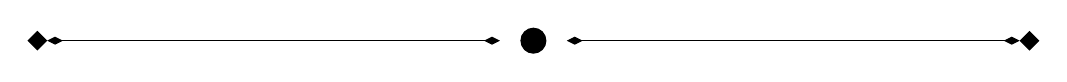
\begin{tikzpicture}[scale = 3]
		\node (a) at (0,0) {};
		\node (b) at (2,0) {};
		\draw[fill] (2.1, 0) circle (1.5pt);
		\node[draw, diamond, fill = black, scale = 0.5] at (0,0) {};
		\node (d) at (2.2,0) {};
		\node (e) at (4.2,0) {};
		\node[draw, diamond, fill = black, scale = 0.5] at (4.2,0) {};
		\draw [{Diamond}-{Diamond}] (a.east) -- (b.west);
		\draw [{Diamond}-{Diamond}] (d.east) -- (e.west);
	\end{tikzpicture}
\end{center}



\end{document}

